\documentclass[11pt, a4paper]{article}
\usepackage[a4paper, margin=2.5cm]{geometry}
\usepackage[utf8]{inputenc}
\usepackage[spanish, es-tabla]{babel}
\usepackage[T1]{fontenc}
\usepackage{lmodern}

\usepackage{amsmath, amsfonts, amssymb}
\usepackage{booktabs}
\usepackage{tabularx}
\usepackage{graphicx}
\usepackage{xcolor}
\usepackage{microtype}
\usepackage{float}
\usepackage{hyperref}

\definecolor{maincolor}{RGB}{30, 64, 175}
\definecolor{accentcolor}{RGB}{37, 99, 235}

\hypersetup{
    colorlinks=true,
    linkcolor=black,
    citecolor=black,
    urlcolor=accentcolor
}

\title{\textbf{\Large Práctica 1: Clasificación de Imágenes de Vehículos mediante Redes Neuronales Convolucionales (CNN)}\\
\large Aprendizaje Automático II -- Curso 2026-27}

\author{
    Carlos Montesdeoca Vega \quad y \quad Aythami Lorenzo Padilla \\
    \small \url{https://github.com/aythamilorenzo/tp1-clasificador-redesconvolucionales-aa2.git}
}

\date{Octubre 2026}

\begin{document}

\maketitle

{
  \vspace{-1cm}
  \renewcommand{\contentsname}{} 
  \tableofcontents
  \vspace{-1cm}
}

\newpage

\section{Introducción y Objetivos}
Este trabajo aborda el diseño, entrenamiento y evaluación de un clasificador de imágenes mediante Redes Neuronales Convolucionales (CNN) en PyTorch. 

Para ello, se ha llevado a cabo un proceso sistemático de búsqueda manual de hiperparámetros comparando un total de nueve configuraciones, organizadas en dos fases: una primera que ajusta hiperparámetros sobre la arquitectura base y una segunda que aborda la normalización de los píxeles, la aumentación de datos y el aprendizaje por transferencia. La búsqueda sobre la arquitectura base no produce ninguna mejora demostrable, mientras que las técnicas de la segunda fase sí, y el aprendizaje por transferencia alcanza un \textbf{99.61\% de precisión} sobre el conjunto de prueba, con 253 aciertos de 254 imágenes.

\section{Descripción del Dataset y Preprocesamiento}
El problema seleccionado consiste en la clasificación de medios de transporte estructurado en 7 clases bien diferenciadas: \textit{auto rickshaws}, \textit{bikes}, \textit{cars}, \textit{motorcycle}, \textit{plane}, \textit{ships} y \textit{trains}. El conjunto contiene 1690 imágenes en total, con una distribución razonablemente equilibrada entre categorías (entre 211 y 256 imágenes por clase).

\subsection{Preprocesamiento}
Para garantizar la homogeneidad en las entradas entregadas a la red convolucional, se aplica la siguiente cadena de transformaciones a cada imagen:
\begin{enumerate}
    \item \textbf{Conversión a espacio RGB:} Se asegura que todas las imágenes tengan 3 canales de color, corrigiendo posibles imágenes en escala de grises o con canal alfa sobrante. Todo esto, con el fin de evitar errores de dimensionalidad en las capas convolucionales.
    \item \textbf{Redimensionado:} Las imágenes se ajustan a una resolución fija de $96 \times 96$ píxeles.
    \item \textbf{Conversión a Tensor:} Se escalan los valores de los píxeles al rango $[0, 1]$.
\end{enumerate}

\subsection{División del Dataset}
El conjunto completo de datos se divide aleatoriamente en tres subconjuntos independientes garantizando la reproducibilidad del proceso mediante una semilla fijada (\texttt{seed = 42}):
\begin{itemize}
    \item \textbf{Entrenamiento (Train) -- 70\%:} 1183 imágenes.
    \item \textbf{Validación (Validation) -- 15\%:} 253 imágenes.
    \item \textbf{Prueba (Test) -- 15\%:} 254 imágenes.
\end{itemize}

La misma semilla se emplea además para la inicialización de los pesos y para el barajado de los lotes durante el entrenamiento. Hay que señalar que esta reproducibilidad es total en CPU, mientras que en GPU, es necesario ajustar algoritmos seleccionados por cuDNN; por ello se fuerza explícitamente el modo determinista mediante \texttt{cudnn.deterministic = True} y \texttt{cudnn.benchmark = False}. Gracias a ello, la repetición de una misma configuración devuelve exactamente los mismos resultados, con la misma precisión decimal.

\section{Arquitectura del Modelo Base (ConvNet)}
La red convolucional propuesta en el modelo base se compone de tres capas convolucionales seguidas de dos capas completamente conectadas (\textit{Fully Connected}).

\begin{table}[H]
\centering
\caption{Estructura detallada de la arquitectura ConvNet base.}
\label{tab:arquitectura}
\begin{tabularx}{\linewidth}{>{\raggedright\arraybackslash}X l l r}
\toprule
\textbf{Capa / Bloque} & \textbf{Configuración} & \textbf{Activación / Operación} & \textbf{Salida} \\
\midrule
Entrada & Imágenes RGB ($96 \times 96$) & -- & $(3, 96, 96)$ \\
Bloque Convolucional 1 & Conv2D(3 $\rightarrow$ 16, $k=5, p=2$) & ReLU + MaxPool2d($2 \times 2$) & $(16, 48, 48)$ \\
Bloque Convolucional 2 & Conv2D(16 $\rightarrow$ 32, $k=5, p=2$) & ReLU + MaxPool2d($2 \times 2$) & $(32, 24, 24)$ \\
Bloque Convolucional 3 & Conv2D(32 $\rightarrow$ 64, $k=5, p=2$) & ReLU + MaxPool2d($2 \times 2$) & $(64, 12, 12)$ \\
Aplanado (Flatten) & Vectorización & -- & $(9216)$ \\
Capa Oculta (FC1) & Linear($9216 \rightarrow 128$) & ReLU + Dropout($p=0.25$) & $(128)$ \\
Capa de Salida (FC2) & Linear($128 \rightarrow 7$) & Lineal (CrossEntropyLoss) & $(7)$ \\
\bottomrule
\end{tabularx}
\end{table}

Conviene señalar que los parámetros no están repartidos de forma uniforme: la capa \texttt{fc1} acumula 1.179.776 pesos, lo que supone el 94.7\% del total de la red (1.245.991). Las tres capas convolucionales, con sus filtros compartidos espacialmente, apenas suman el 5.3\%. Este desequilibrio es una consecuencia directa del aplanado, que entrega 9216 valores a una única capa densa sin ninguna compartición.

\subsection{Estrategia de Parada Anticipada (Early Stopping)}
Para prevenir el sobreajuste se monitoriza la pérdida de validación (\textit{Validation Loss}) al término de cada época. Se define una paciencia inicial de 5 épocas (\texttt{patience = 5}). Si la pérdida de validación no mejora respecto al mínimo histórico alcanzado, el contador aumenta; si el contador llega al límite de la paciencia, el entrenamiento se interrumpe.

Durante todo el proceso, cada vez que la pérdida de validación alcanza un nuevo mínimo histórico se guardan los pesos del modelo en el archivo \texttt{best\_conv\_model.pth}. Esos son los pesos con los que se evalúa posteriormente el modelo sobre el conjunto de prueba, de modo que la evaluación final no utiliza el estado final de la red sino su punto óptimo de generalización.

La paciencia no se mantiene fija en todos los experimentos: al reducirse la tasa de aprendizaje en el Experimento 2 hubo que ampliarla, porque un paso más pequeño tarda más en encontrar un mínimo nuevo y con el valor original el entrenamiento se habría cortado antes de llegar a él.

\section{Plan de Búsqueda de Hiperparámetros}
Se comparan un total de 9 configuraciones distintas. En cada una, lo que se hace es \textbf{cambiar una sola variable cada vez respecto al modelo base}: todas las configuraciones arrancan de los mismos pesos iniciales y la misma arquitectura del Experimento 1, de modo que cualquier diferencia observada en los resultados pueda atribuirse al hiperparámetro que se ha modificado. La alternativa de ir acumulando cambios sobre la configuración mejor hasta el momento se descartó, ya que con un conjunto de test de 254 imágenes las diferencias pequeñas son indistinguibles del ruido y encadenar decisiones sobre ellas conduciría a elegir el camino por azar.

El estudio se organiza en dos fases. La primera recorre los hiperparámetros clásicos de la red y está recogida en la Tabla~\ref{tab:experimentos}. La segunda, recogida en la Tabla~\ref{tab:experimentos_datos}, aborda mejoras que no son ajustes de un hiperparámetro sino cambios en los datos de entrada y en el propio modelo: la normalización de los píxeles, data augmentation, y transfer learning. Se deja para el final porque son, precisamente, los métodos que atacan la causa del problema detectado en la primera fase, dónde vimos que el cuello de botella de la red no era una cuestión de hiperparámetros sino la cantidad de datos disponibles.

\begin{table}[H]
\centering
\footnotesize
\caption{Tabla comparativa del plan de experimentos de hiperparámetros. En negrita, el hiperparámetro que varía cada configuración respecto al modelo base. \textbf{Ép.} es el número máximo de épocas y \textbf{Pac.} la paciencia del \textit{Early Stopping}.}
\label{tab:experimentos}
\setlength{\tabcolsep}{3pt}
\begin{tabularx}{\linewidth}{c X c c c c c c r}
\toprule
\textbf{Exp.} & \textbf{Capas conv.} & \textbf{Neu. FC1} & \textbf{Ép.} & \textbf{Pac.} & \textbf{LR} & \textbf{Batch} & \textbf{Act.} & \textbf{Acc. Test} \\
\midrule
\textbf{1} & 3 (16, 32, 64) & 128 & 15 & 5 & 0.001 & 32 & ReLU & \textbf{87.80\%} \\
\textbf{2} & 3 (16, 32, 64) & 128 & 50 & 10 & \textbf{0.0001} & 32 & ReLU & \textbf{88.98\%} \\
\textbf{3} & \textbf{4 (16, 32, 64, 128)} & 128 & 50 & 5 & 0.001 & 32 & ReLU & 84.25\% \\
\textbf{4} & 3 (16, 32, 64) & 128 & 50 & 5 & 0.001 & \textbf{64} & ReLU & \textbf{90.55\%} \\
\textbf{5} & 3 (16, 32, 64) & 128 & 50 & 5 & 0.001 & 32 & \textbf{LeakyReLU} & 87.01\% \\
\textbf{6} & 3 (16, 32, 64) & \textbf{32} & 50 & 5 & 0.001 & 32 & ReLU & 83.07\% \\
\bottomrule
\end{tabularx}
\setlength{\tabcolsep}{6pt}
\end{table}

En el Experimento 2 los valores de épocas y paciencia varían de forma conjunta con la tasa de aprendizaje, ya que los tres son dependientes entre sí: reducir la tasa de aprendizaje sin aumentar las iteraciones dejaría el modelo a medias y la comparación carecería de sentido. El optimizador se mantiene fijo (\textbf{Adam}) en las nueve configuraciones para aislar el efecto del resto de hiperparámetros.

Se descartó además utilizar el mismo número de épocas para cada configuración. Cuando una red tarda más en converger, por ser más profunda o por llevar un tamaño de lote mayor que reduce los pasos de gradiente por época, un número pequeño de épocas podría cortar el entrenamiento a medias y la comparación dejaría de ser justa. Por eso el número se fija de forma generosa y es el \textit{Early Stopping}, y no el número de épocas, quién decide cuándo termina cada experimento. 

En todos los casos la selección del mejor punto de parada se realiza sobre la pérdida de validación, sin inspeccionar nunca el conjunto de prueba hasta la evaluación final.

\begin{table}[H]
\centering
\footnotesize
\caption{Tabla comparativa de la segunda fase, sobre los datos de entrada y el modelo. Los Experimentos 7 y 8 conservan la resolución de $96 \times 96$ y la arquitectura del modelo base, de modo que la única diferencia respecto al Experimento 1 es el preprocesamiento. El Experimento 9 sí cambia de arquitectura y de resolución a la vez.}
\label{tab:experimentos_datos}
\setlength{\tabcolsep}{3pt}
\begin{tabularx}{\linewidth}{c X X c c}
\toprule
\textbf{Exp.} & \textbf{Cambio respecto al modelo base} & \textbf{Resolución} & \textbf{Ép.} & \textbf{Acc. Test} \\
\midrule
\textbf{7} & Añadir \texttt{transforms.Normalize} & $96 \times 96$ & 50 & 88.98\% \\
\textbf{8} & Data augmentation solo en entrenamiento & $96 \times 96$ & 50 & 91.73\% \\
\textbf{9} & Transfer Learning con ResNet-18 preentrenada & $224 \times 224$ & 50 & \textbf{99.61\%} \\
\bottomrule
\end{tabularx}
\setlength{\tabcolsep}{6pt}
\end{table}

\section{Resultados Experimentales}

\subsection{Experimento 1: modelo base}
El primer experimento se ejecutó utilizando el optimizador \textbf{Adam} con una tasa de aprendizaje $\eta = 0.001$, un tamaño de lote de 32 imágenes y un máximo de 15 épocas con una paciencia de 5.

\subsubsection{Evolución del entrenamiento}
El mecanismo de parada anticipada se activó en la \textbf{época 10}, tras cinco épocas consecutivas sin mejorar la pérdida de validación. No obstante, el mínimo histórico de dicha pérdida se alcanzó en la \textbf{época 5}, que es el punto cuyos pesos se conservaron para la evaluación posterior. La Tabla~\ref{tab:resultados_exp1} recoge las métricas medidas sobre ese mismo punto óptimo, de modo que las tres filas corresponden a un único modelo.

\begin{table}[H]
\centering
\caption{Métricas obtenidas en el Experimento 1 (Modelo Base), medidas sobre los pesos de la época 5.}
\label{tab:resultados_exp1}
\begin{tabular}{l c c}
\toprule
\textbf{Conjunto de Datos} & \textbf{Pérdida (Loss)} & \textbf{Precisión (Accuracy)} \\
\midrule
Entrenamiento & 0.4249 & 85.21\% \\
Validación & 0.5032 & 81.82\% \\
\textbf{Prueba (Test)} & \textbf{0.4141} & \textbf{87.80\%} \\
\bottomrule
\end{tabular}
\end{table}

\begin{figure}[H]
\centering
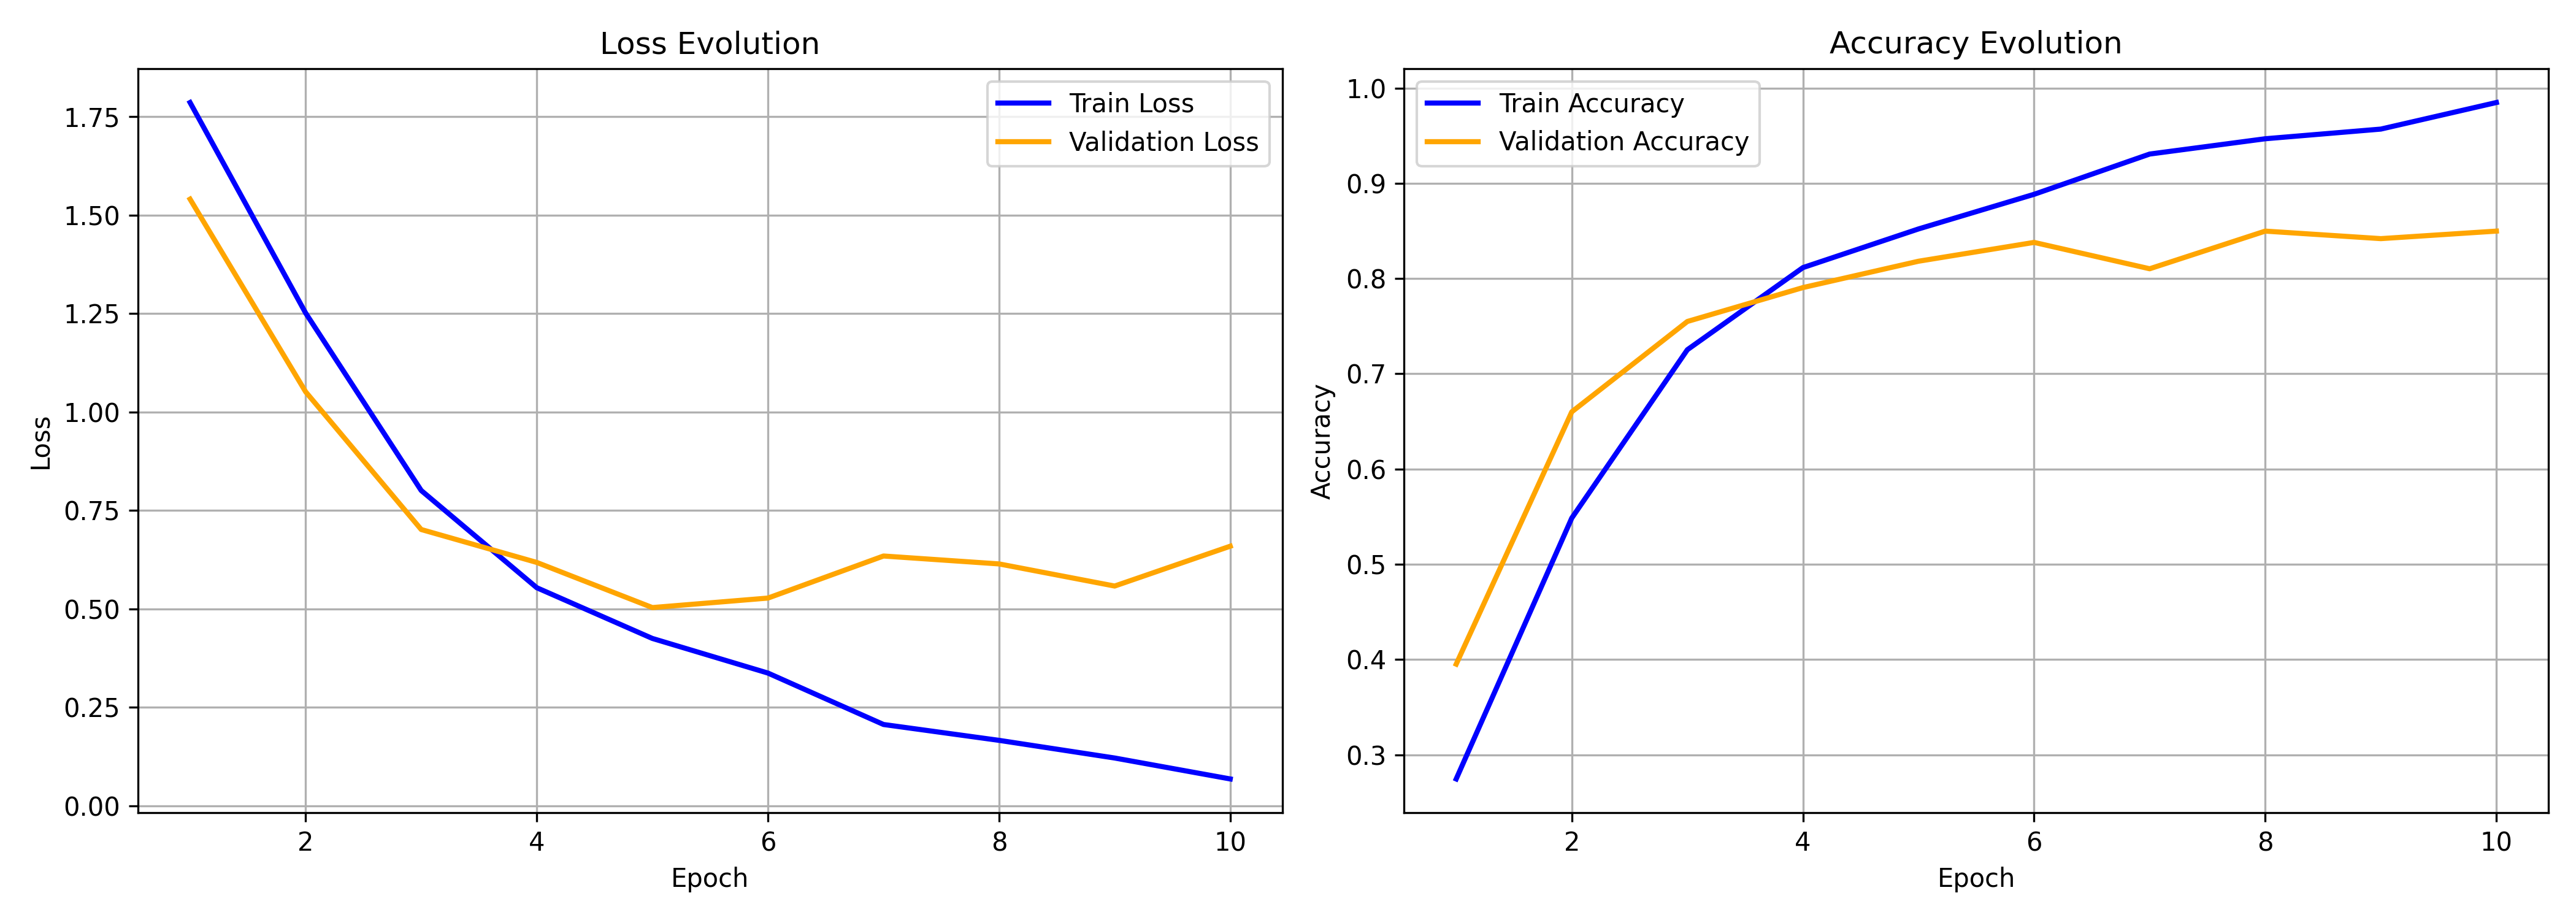
\includegraphics[width=0.90\linewidth]{../results/config1_baseline/training_history.png}
\caption{Evolución de la pérdida y precisión en entrenamiento y validación (Experimento 1).}
\label{fig:curvas_exp1}
\end{figure}

Como se aprecia en la Figura~\ref{fig:curvas_exp1}, la precisión de entrenamiento sigue creciendo de forma sostenida hasta superar el 98\%, mientras que la de validación se estabiliza entre el 82\% y el 85\%. A partir de la quinta época la brecha entre ambas curvas se ensancha de manera consistente: la pérdida de validación deja de mejorar mientras la de entrenamiento continúa descendiendo. Este comportamiento sugiere que a partir de la época 5, la red comienza a sobreajustarse y justifica la intervención de la parada anticipada, que actúa antes de que la red llegue a memorizar el conjunto de entrenamiento.

En el punto óptimo seleccionado la diferencia entre ambas precisiones es de apenas 3.4 puntos, lo que indica que el modelo aún generaliza correctamente en el instante en que se detiene el entrenamiento.

\subsubsection{Evaluación en el conjunto de test}
Tras la evaluación aislada sobre el conjunto de test utilizando los mejores pesos guardados, el modelo alcanzó una precisión del \textbf{87.80\%}, superando el objetivo fijado del 85\%.

La precisión medida sobre el conjunto de prueba resulta superior a la registrada en validación. 

\begin{figure}[H]
\centering
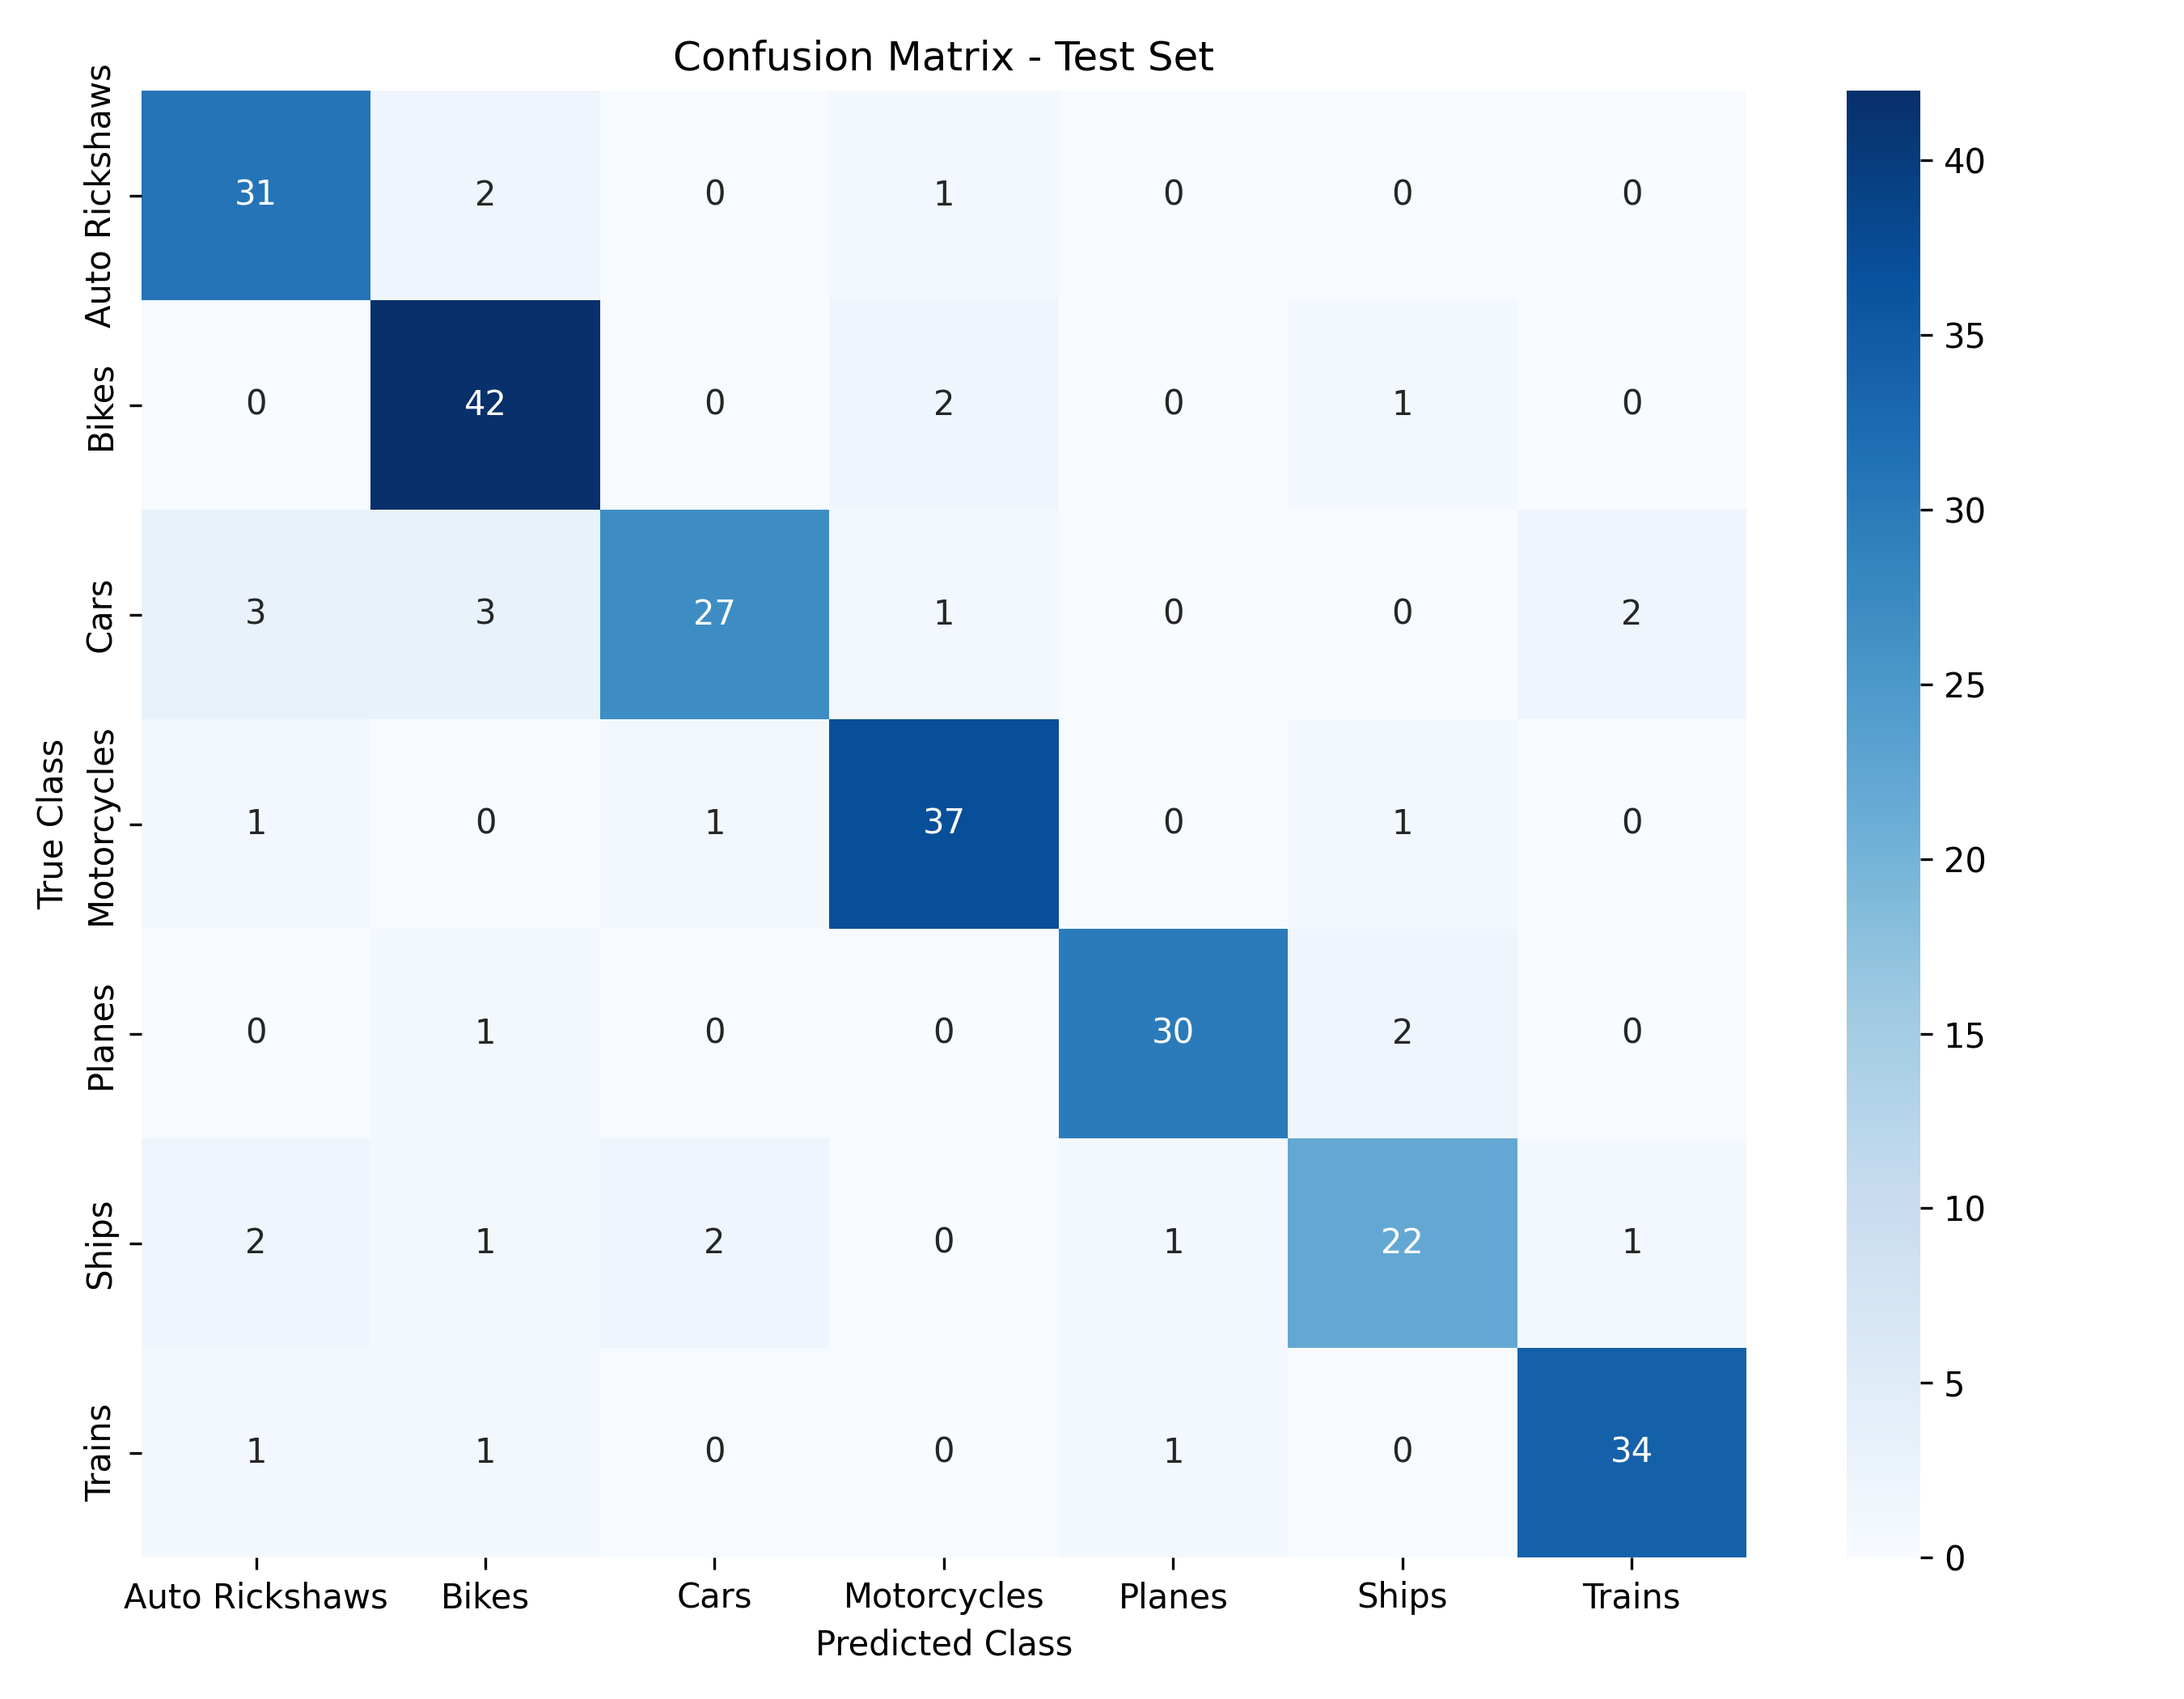
\includegraphics[width=0.65\linewidth]{../results/config1_baseline/test_confusion_matrix.png}
\caption{Matriz de confusión obtenida sobre el conjunto de test (Experimento 1).}
\label{fig:matriz_confusion_exp1}
\end{figure}

El análisis de la matriz de confusión permite extraer las siguientes conclusiones sobre las 7 categorías:
\begin{itemize}
    \item \textbf{Clases con alto rendimiento:} Las categorías con patrones geométricos distintivos como \textit{plane}, \textit{ships} y \textit{trains} presentan tasas de acierto elevadas.
    \item \textbf{Confusiones principales:} Se observan ligeras confusiones entre clases visualmente similares como \textit{bikes} frente a \textit{motorcycle}, así como entre \textit{auto rickshaws} y \textit{cars} debido a la presencia de contextos urbanos parecidos.
\end{itemize}

\subsection{Experimento 2: tasa de aprendizaje reducida}
En este segundo experimento lo único que se modifica respecto al modelo base es la tasa de aprendizaje del optimizador, que pasa de $\eta = 0.001$ a $\eta = 0.0001$, es decir, un orden de magnitud por debajo. Como el paso del gradiente se reduce diez veces, el modelo necesita muchas más iteraciones para recorrer la misma distancia, por lo que se amplía de forma asociada el número de épocas (de 15 a 50) y la paciencia (de 5 a 10).

El entrenamiento se detuvo en la \textbf{época 48}, habiendo alcanzado el mínimo histórico de pérdida de validación en la \textbf{época 38}. Las métricas de la Tabla~\ref{tab:resultados_exp2} corresponden a ese punto.

\begin{table}[H]
\centering
\caption{Métricas obtenidas en el Experimento 2 (tasa de aprendizaje 0.0001), medidas sobre los pesos de la época 38.}
\label{tab:resultados_exp2}
\begin{tabular}{l c c}
\toprule
\textbf{Conjunto de Datos} & \textbf{Pérdida (Loss)} & \textbf{Precisión (Accuracy)} \\
\midrule
Entrenamiento & 0.1574 & 94.76\% \\
Validación & 0.4813 & 85.38\% \\
\textbf{Prueba (Test)} & \textbf{0.3778} & \textbf{88.98\%} \\
\bottomrule
\end{tabular}
\end{table}

\begin{figure}[H]
\centering
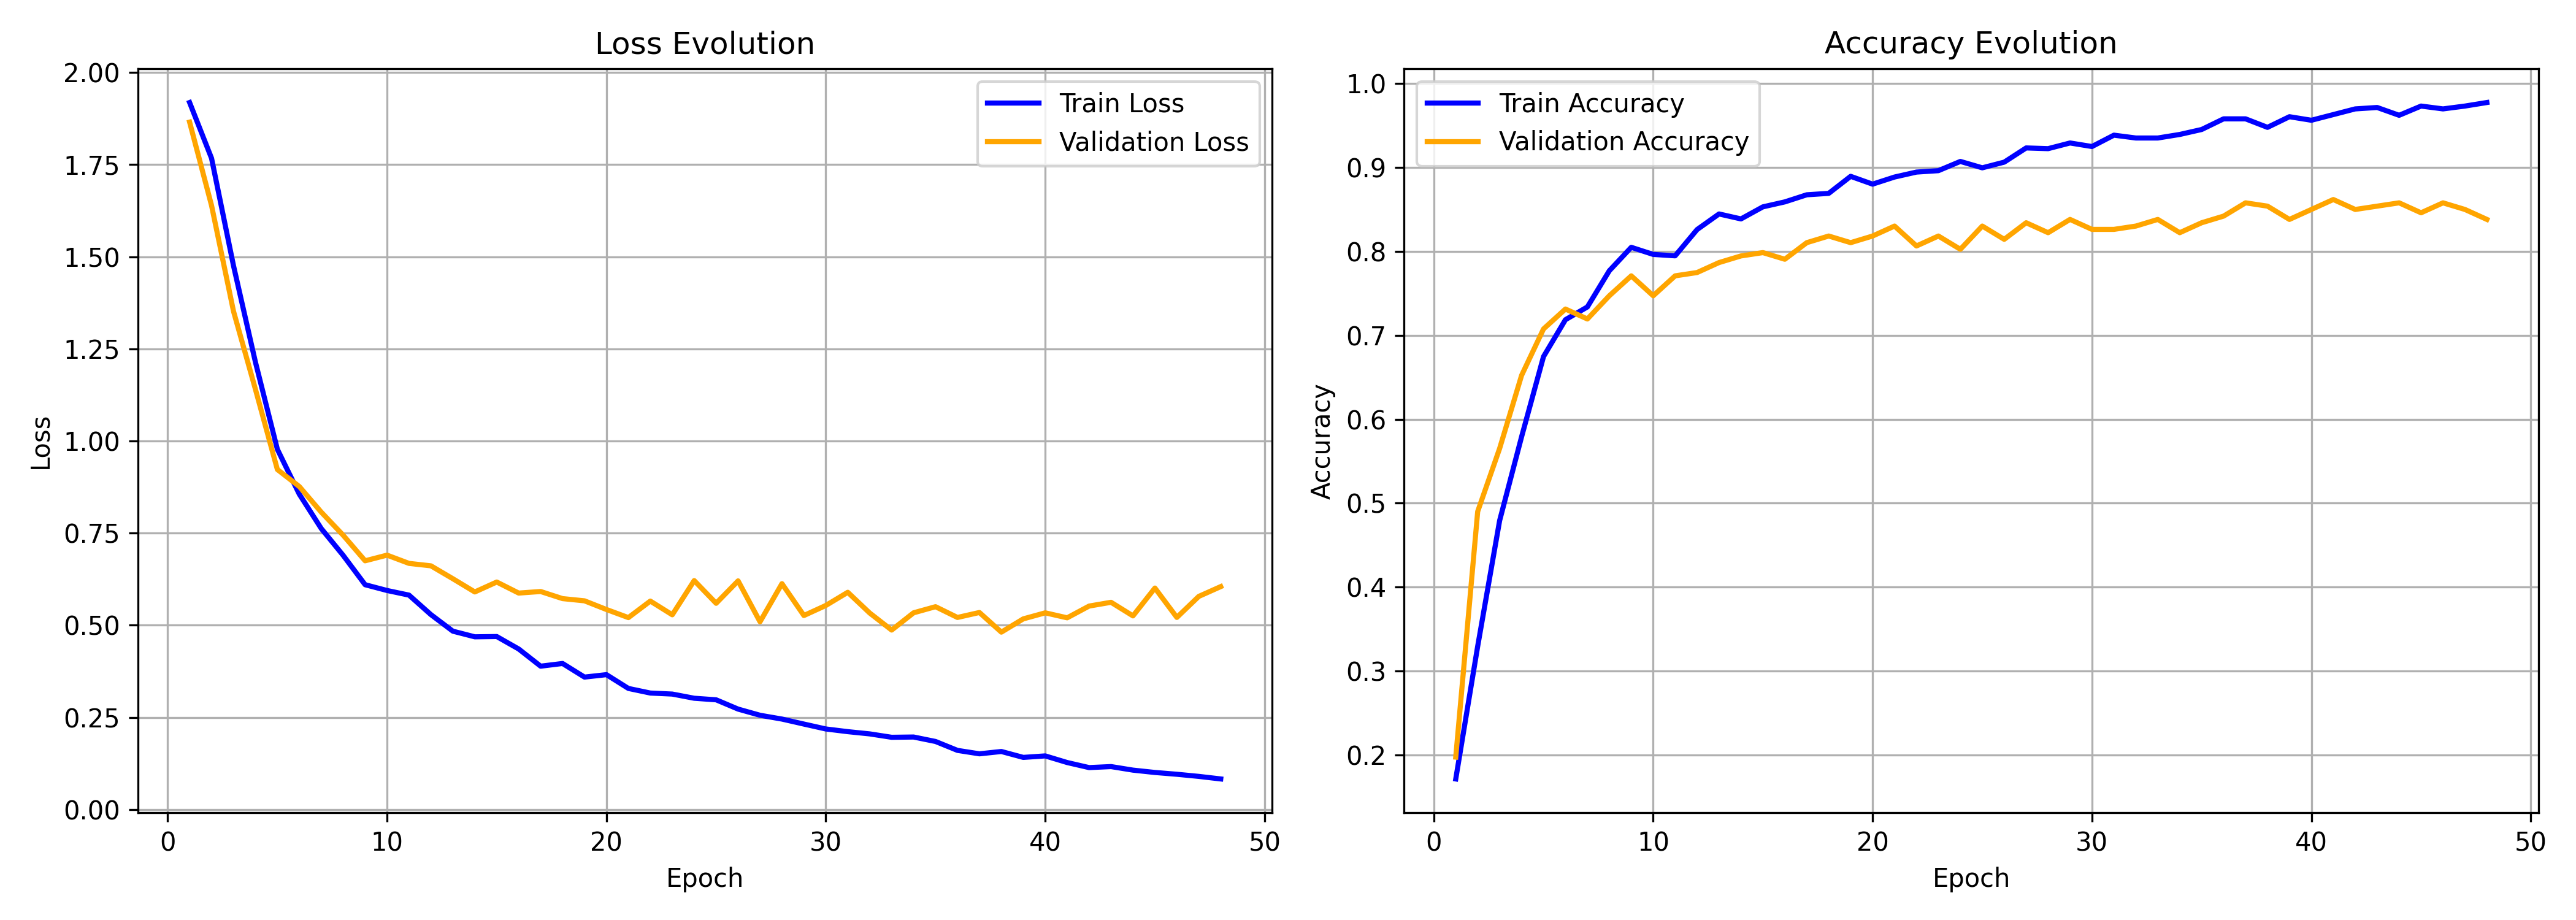
\includegraphics[width=0.90\linewidth]{../results/config2_lr0001/training_history.png}
\caption{Evolución de la pérdida y precisión en entrenamiento y validación (Experimento 2).}
\label{fig:curvas_exp2}
\end{figure}

\subsubsection{Comportamiento de la pérdida de validación}
La curva del Experimento 2 se comporta de forma notablemente distinta a la del modelo base. Mientras que con $\eta = 0.001$ la pérdida de validación alcanzaba su mínimo en la época 5 y a partir de ahí subía de forma prácticamente monótona, con $\eta = 0.0001$ la curva desciende mucho más despacio y, una vez que se estabiliza alrededor de la época 20, \textbf{oscila} entre 0.48 y 0.62 en lugar de divergir limpiamente.

Con 'pasos' diez veces más pequeños la red no abandona la zona del mínimo, sino que da tirones pequeños por los alrededores, y de vez en cuando da con una configuración de pesos que resulta favorable. Se produjeron así varios descensos bruscos que reiniciaron el contador de la paciencia, en concreto en las épocas 27, 33 y 38.

Esto es una prueba de que la paciencia ampliada fue un detalle importante, ya que si repitiéramos la simulación con la paciencia original de 5, el entrenamiento se habría cortado en la \textbf{época 26}, una sola época antes del primero de esos descensos, y el modelo conservado habría sido el de la época 21 con una pérdida de validación de 0.5207. Con la paciencia de 10 se llegó hasta el mínimo de 0.4813 de la época 38. Esto demuestra por qué la tasa de aprendizaje, el número de épocas y la paciencia tienen que ajustarse juntos.

En cualquier caso, la red se sigue sobreajustando conforme avanzan las épocas: en la época 48 la precisión de entrenamiento era del 97.72\% frente al 83.79\% de validación, una brecha de casi 14 puntos. Simplemente que con 'pasos' pequeños el camino hasta ese punto es más largo.

\subsubsection{Comparación con el modelo base}
El Experimento 2 mejora el modelo base en todas las métricas registradas: la pérdida de validación baja de 0.5032 a 0.4813, la precisión de validación sube de 81.82\% a 85.38\% y la precisión de test pasa de 87.80\% a 88.98\%.

Sin embargo, conviene no sobrevalorar esa última cifra. Ya que la división del conjunto de prueba es fija, ambos experimentos evalúan sobre las mismas \textbf{254 imágenes}, siendo que el experimento base acierta en 223 y este en 226, una diferencia tan pequeña que no es significativa y se le puede atribuir al ruido teniendo en cuenta el tamaño del conjunto de datos.

\subsection{Experimento 3: red más profunda}

El tercer experimento añade una cuarta capa convolucional con 128 filtros, con el mismo tamaño de kernel y padding que las anteriores. El número de neuronas de la capa densa se mantiene en 128, de modo que la profundidad es el único hiperparámetro que cambia respecto al modelo base.

Al introducir un cuarto bloque de submuestreo, el vector que llega a la capa densa pasa de 9216 a 4608 elementos, y al mantener las 128 neuronas el número de parámetros de \texttt{fc1} se reduce a la mitad, de 1.179.648 a 589.824. En conjunto la red \textbf{no crece sino que encoge}: baja de 1.245.991 a 861.095 parámetros, un 31\% menos. El experimento mide por tanto el efecto de una red más profunda y a la vez más ligera.

En la primera ejecución, se estableció un número de 15 épocas heredadas del modelo base y resultó insuficiente: en la última época la pérdida de validación acababa de alcanzar su mínimo histórico (0.3839) y el contador de la paciencia estaba a cero, de forma que el corte no lo produjo el \textit{Early Stopping} sino el número de épocas. Se amplió dicho número a 50 épocas dejando intacta la paciencia. Con ese margen el entrenamiento se detuvo en la época 20, sin que se mejorara nunca el mínimo de la época 15, con lo que los pesos conservados y las métricas finales quedaron exactamente igual. 

\begin{table}[H]
\centering
\caption{Métricas obtenidas en el Experimento 3 (red de cuatro capas convolucionales), medidas sobre los pesos de la época 15.}
\label{tab:resultados_exp3}
\begin{tabular}{l c c}
\toprule
\textbf{Conjunto de Datos} & \textbf{Pérdida (Loss)} & \textbf{Precisión (Accuracy)} \\
\midrule
Entrenamiento & 0.0825 & 97.04\% \\
Validación & 0.3839 & 88.14\% \\
\textbf{Prueba (Test)} & \textbf{0.6654} & \textbf{84.25\%} \\
\bottomrule
\end{tabular}
\end{table}

\subsubsection{Una validación excelente y un test discrepante}

 En validación la configuración 3 es \textbf{la mejor de las tres}: registra la pérdida más baja (0.3839 frente a 0.4813 y 0.5032) y la precisión más alta (88.14\% frente a 85.38\% y 81.82\%). Sin embargo, sobre el conjunto de prueba es \textbf{la peor}, con un 84.25\% frente al 87.80\% y al 88.98\% de los experimentos anteriores.

Esto puede atribuirse a simple ruido muestral, los conjuntos de validación y de prueba son muestras independientes de tamaños comparables, 253 y 254 imágenes, de modo que el propio desajuste entre ambos tiene un margen de error de unos cuatro puntos. Para apreciar cuánto se mueve por sí solo basta comparar con el modelo base, donde la diferencia va en el sentido contrario: 81.82\% en validación frente al 87.80\% en prueba. Entre las dos configuraciones el desajuste varía en más de nueve puntos sin que ninguna haya cambiado de estrategia de entrenamiento, y esa oscilación es precisamente la magnitud que cabe esperar del ruido de muestreo a ese tamaño.

\subsection{Experimento 4: tamaño de lote}

El cuarto experimento duplica el tamaño de lote de 32 a 64 imágenes. Es el único hiperparámetro que cambia respecto al modelo base.

Duplicar el lote tiene una consecuencia directa: el número de pasos de gradiente por época se reduce a la mitad, de 37 a 18. Es decir, en cada época el modelo se actualiza la mitad de veces. Por eso el número de épocas se mantiene mayor (50): si se hubiera dejado el tope del modelo base, estaríamos comparando una configuración con el doble de actualizaciones que otra, y el resultado no diría nada sobre el tamaño de lote.

El entrenamiento se detuvo en la época 14 y el mínimo de la pérdida de validación se alcanzó en la \textbf{época 9}.

\begin{table}[H]
\centering
\caption{Métricas obtenidas en el Experimento 4 (tamaño de lote 64), medidas sobre los pesos de la época 9.}
\label{tab:resultados_exp4}
\begin{tabular}{l c c}
\toprule
\textbf{Conjunto de Datos} & \textbf{Pérdida (Loss)} & \textbf{Precisión (Accuracy)} \\
\midrule
Entrenamiento & 0.1968 & 93.66\% \\
Validación & 0.4834 & 86.56\% \\
\textbf{Prueba (Test)} & \textbf{0.3595} & \textbf{90.55\%} \\
\bottomrule
\end{tabular}
\end{table}

\subsubsection{Análisis de los resultados}

Cuando se aumenta el tamaño de lote, en general, esto conduce a converger hacia mínimos de manera más rápida ya que al promediar el error de más muestras, la varianza es menor y se obtiene una estimación más precisa de la dirección real hasta el mínimo. Sin embargo, esto puede ser un arma de doble filo, ya que cuando aumentamos el tamaño de lote, el ruido disminuye, y la red puede instalarse con más facilidad en mínimos locales; de lo contrario, cuando tenemos lotes más pequeños, ese ruido muchas veces actúa como mecanismo regularizador y puede ayudar a la red a generalizar mejor, llegando hacia mínimos anchos. En la práctica, sin embargo, esta configuración obtiene la \textbf{mejor precisión de todo el estudio}, un 90.55\%.

Dos razones explican este resultado:

En primer lugar, el ruido que anteriormente se atribuía al lote pequeño ya no hacía falta. La red incorpora por su cuenta dos mecanismos de regularización, \texttt{Dropout} con $p=0.25$ y el \textit{Early Stopping}, y con ambos presentes el sobreajuste se mantiene controlado sin necesidad de la ayuda del ruido de muestreo. 

En segundo lugar, tal y como se comentaba anteriormente, cada actualización se estima con el doble de muestras, de modo que apunta más en la dirección del gradiente real. Hay menos pasos, pero cada uno es más certero.

\subsection{Experimento 5: función de activación}

El quinto experimento sustituye la función \texttt{ReLU} por \texttt{LeakyReLU} en las cuatro activaciones de la red, tanto en las capas convolucionales como en la primera capa densa. El resto de hiperparámetros coincide con el modelo base.

La diferencia entre ambas es mínima en la fórmula y relevante en el comportamiento. \texttt{ReLU} anula por completo los valores negativos; \texttt{LeakyReLU} les aplica una pendiente del 1\%. De manera que, con \textbf{ReLU}, cuando una neurona recibe entradas negativas, la salida y gradiente de esta quedan en 0, de modo que la neurona no aprende. Con \textbf{LeakyReLU}, conserva un pequeño gradiente que le permite seguir aprendiendo.

\begin{table}[H]
\centering
\caption{Métricas obtenidas en el Experimento 5 (activación LeakyReLU), medidas sobre los pesos de la época 6.}
\label{tab:resultados_exp5}
\begin{tabular}{l c c}
\toprule
\textbf{Conjunto de Datos} & \textbf{Pérdida (Loss)} & \textbf{Precisión (Accuracy)} \\
\midrule
Entrenamiento & 0.1647 & 94.08\% \\
Validación & 0.5471 & 82.21\% \\
\textbf{Prueba (Test)} & \textbf{0.4736} & \textbf{87.01\%} \\
\bottomrule
\end{tabular}
\end{table}

\subsubsection{No-diferencia medible}

La hipótesis de partida era que a esta escala el problema de las neuronas muertas no llegaría a manifestarse: con 128 neuronas en la capa densa, inicialización estándar y optimizador Adam, era de esperar que pocas neuronas quedaran inactivas de forma permanente, y por tanto que el efecto de \texttt{LeakyReLU} fuera escaso.

Así fue. Sobre el conjunto de prueba esta configuración acierta 221 de las 254 imágenes, frente a las 223 del modelo base, la diferencia es de \textbf{dos imágenes}.

El resultado concluyente es que \textbf{la función de activación no es un factor determinante en una red de este tamaño}. Dicho de otro modo: el problema de las neuronas muertas, aunque real, no llega a pesar lo suficiente como para alterar la precisión final cuando la red ya dispone de dropout y early stopping.

\subsubsection{Un efecto secundario en la dinámica del entrenamiento}

Donde sí se nota el cambio es en la velocidad. Esta configuración alcanza el 94.08\% de precisión de entrenamiento en la \textbf{época 6}, antes que ninguna otra del estudio, y se detiene en la época 11. Una posible explicación es que, al dejar pasar gradiente a través de los valores negativos, las neuronas no quedan inactivas y el modelo puede ajustarse más rápido.

El problema es que ese mismo empujón acelera la memorización. En el punto óptimo, la época 6, la brecha entre la precisión de entrenamiento y la de validación es de \textbf{11.87 puntos}, la \textbf{mayor} de las nueve configuraciones. Además registra la \textbf{peor pérdida de validación de todo el estudio}, 0.5471 frente al 0.3839 del Experimento 3.

En resumen, \texttt{LeakyReLU} aceleró tanto el aprendizaje como el sobreajuste, y en 1183 imágenes de entrenamiento la parada anticipada llegó pronto. El resultado final no mejora, pero la dinámica sí cambia.

\subsection{Experimento 6: número de neuronas en la capa densa}

En este caso, se reduce el número de neuronas de la primera capa densa de 128 a 32. Es el hiperparámetro que más pesa en el modelo: con 128 neuronas y un vector de entrada de 9216 valores, esa sola capa acumula 1.179.648 parámetros, el 94.7\% de la red entera, mientras que las tres capas convolucionales apenas suman 65.104 parámetros. Con 32 neuronas el modelo queda en 360.487 parámetros, un 71\% menos que el modelo base.

La pregunta que abre este experimento es la siguiente: ¿hace falta toda esa capacidad inicial, o sobra y es la causante del sobreajuste?

\begin{table}[H]
\centering
\caption{Métricas obtenidas en el Experimento 6 (capa densa de 32 neuronas), medidas sobre los pesos de la época 7.}
\label{tab:resultados_exp6}
\begin{tabular}{l c c}
\toprule
\textbf{Conjunto de Datos} & \textbf{Pérdida (Loss)} & \textbf{Precisión (Accuracy)} \\
\midrule
Entrenamiento & 0.5688 & 78.61\% \\
Validación & 0.4937 & 82.61\% \\
\textbf{Prueba (Test)} & \textbf{0.5205} & \textbf{83.07\%} \\
\bottomrule
\end{tabular}
\end{table}

\begin{figure}[H]
\centering
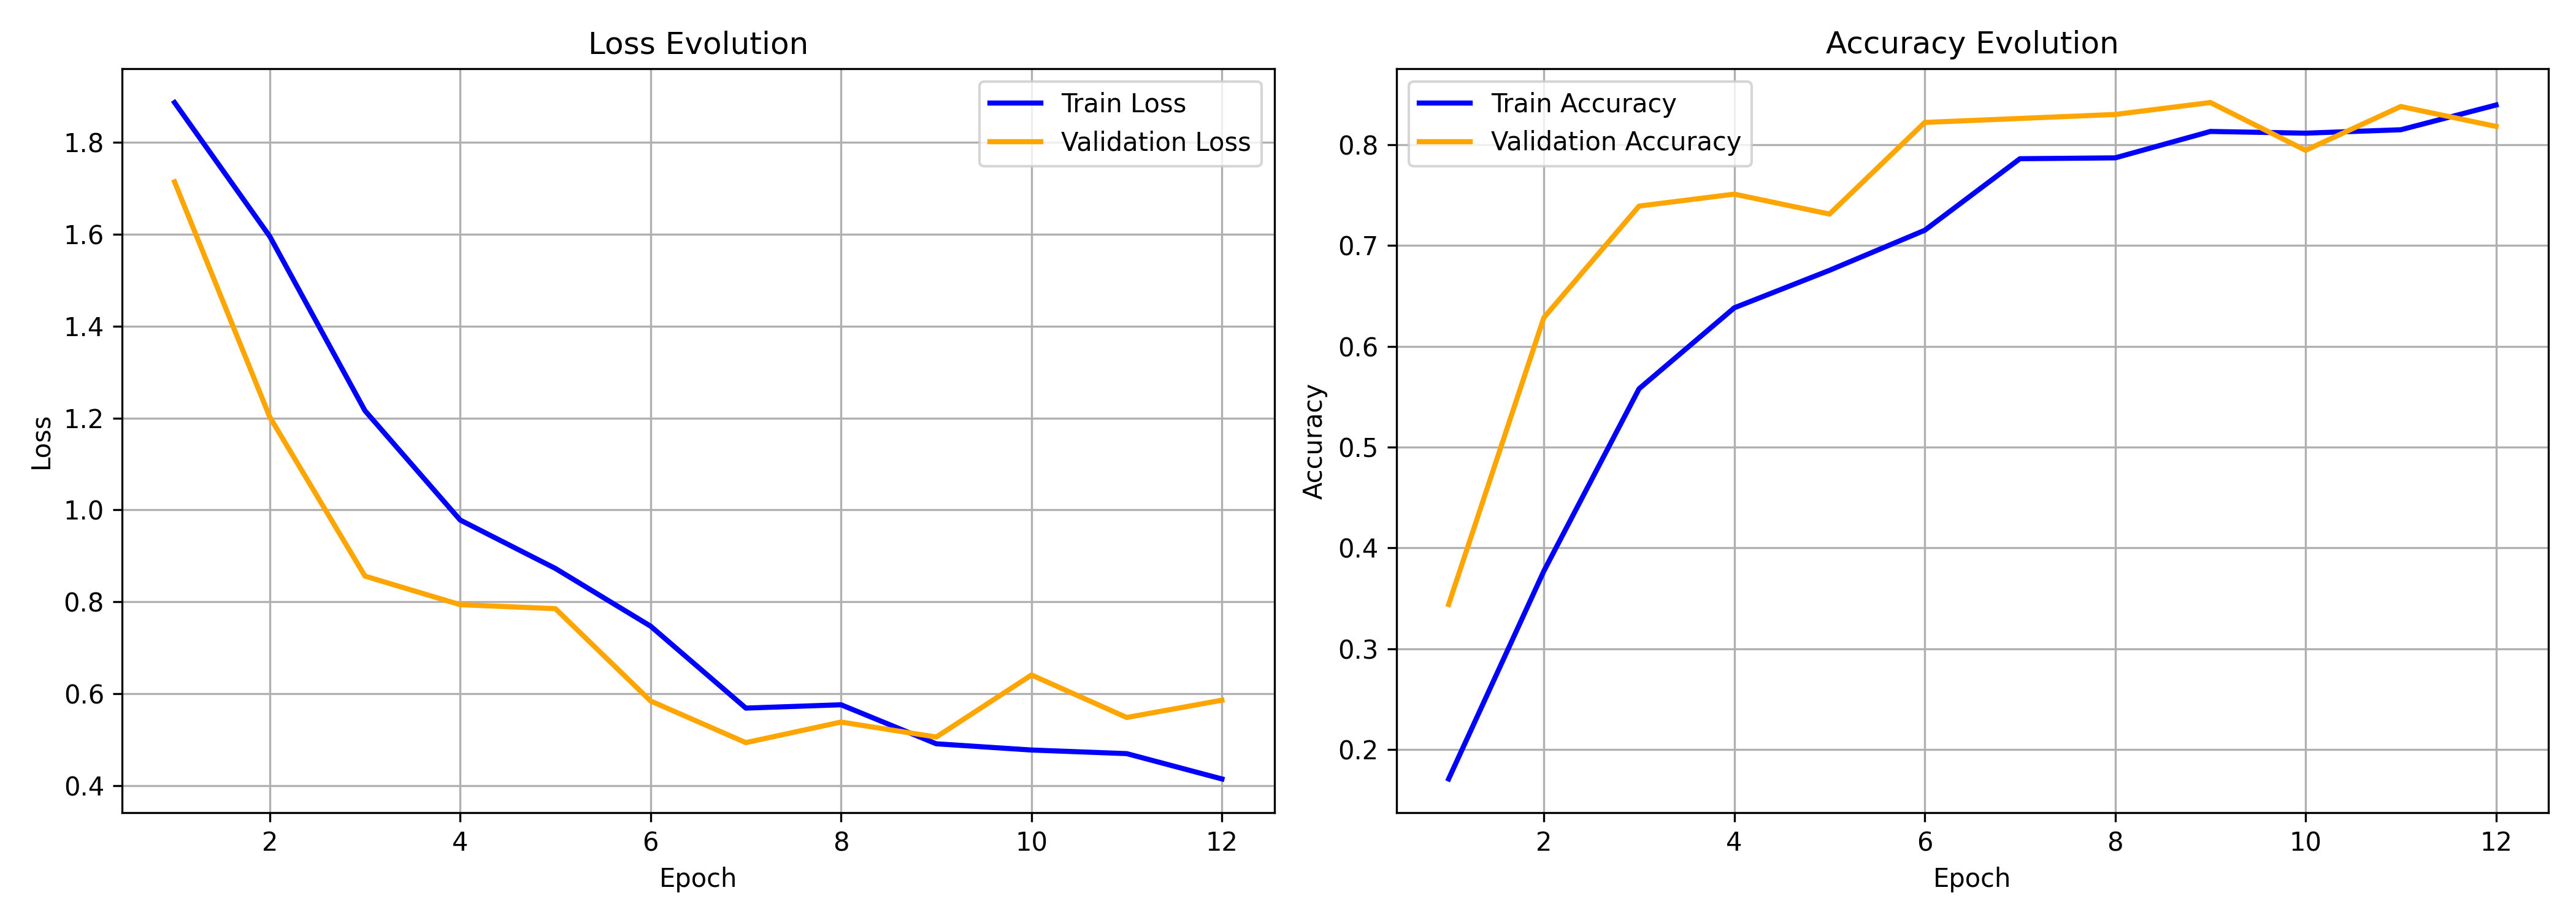
\includegraphics[width=0.90\linewidth]{../results/config6_fc32/training_history.png}
\caption{Evolución de la pérdida y precisión en entrenamiento y validación (Experimento 6). Nótese que la curva de entrenamiento se queda por debajo de la de validación, comportamiento contrario al de los cinco experimentos anteriores.}
\label{fig:curvas_exp6}
\end{figure}

\subsubsection{Infraajuste: la señal más nítida del experimento}

La respuesta es que \textbf{no sobraba capacidad}, y el experimento lo demuestra con la señal más clara de las seis. En el punto óptimo, la época 7, la precisión de entrenamiento es del 78.61\% y la de validación del 82.61\%: la primera es \textbf{menor} que la segunda. Es la única configuración de todo el estudio en la que la brecha entre ambos conjuntos resulta negativa, de $-4.00$ puntos, mientras que en las otras cinco va de +3.39 a +11.87.

Una precisión de entrenamiento por debajo de la de validación sugiere de manera clara que hay \textbf{infraajuste}: al modelo le falta capacidad y ni siquiera sobre los datos que está viendo logra un buen resultado. El \texttt{Dropout} contribuye a esa inversión, porque está activo durante el entrenamiento y se desactiva al evaluar, pero no la explica por sí solo. Lo relevante es que en todas las demás configuraciones la relación iba al revés y la cuestión era cuánto sobreajustaba, no si alcanzaba.

En resumen, la precisión de entrenamiento confirma la lectura. Donde el modelo base llegaba al 98\% y el Experimento 3 al 97.04\%, aquí se detiene en el 78.61\%, muy por debajo incluso de lo que obtiene en validación.

\subsubsection{Resultado y significancia}

Esta configuración obtiene el \textbf{último lugar}, con un 83.07\% de precisión en el conjunto de prueba. Frente a la mejor configuración del estudio, el Experimento 4, la desventaja es de \textbf{diecinueve imágenes} sobre 254.

Al inicio del informe se observó que la distribución de parámetros del modelo era muy desigual: el 94.7\% se concentraba en una única capa densa y apenas el 5.2\% en las capas convolucionales que procesan la imagen. Este experimento responde a la duda que dejó esa observación. \textbf{La capacidad de esa capa se estaba usando}, y reducirla no regulariza al modelo sino que lo empobrece. La conclusión práctica es que el desequilibrio, aunque llamativo, no es un defecto a corregir: es una consecuencia del aplanado y la arquitectura funciona correctamente con él.

\subsection{Experimento 7: normalización de los píxeles}

Los seis experimentos anteriores entregan a la red valores de píxel en el rango $[0, 1]$, sin más ajuste. Este séptimo experimento añade un paso final al flujo de preprocesamiento, \texttt{transforms\allowbreak.Normalize}, que resta a cada canal su media y divide por su desviación típica. Los valores empleados son los de \textbf{ImageNet}, $\mu = (0.485, 0.456, 0.406)$ y $\sigma = (0.229, 0.224, 0.225)$, y no los calculados sobre el propio conjunto. Esta decisión responde a dos motivos: son los que exigen las redes preentrenadas, de manera que el Experimento 9 queda aislado y su efecto puede atribuirse al modelo y no al preprocesamiento, y al ser idénticos en todas las imágenes no dependen de ninguna decisión tomada sobre los datos.

La imagen no cambia de contenido, pero su representación numérica pasa de estar sesgada hacia valores positivos pequeños a estar centrada en cero.

\begin{table}[H]
\centering
\caption{Métricas obtenidas en el Experimento 7 (normalización), medidas sobre los pesos de la época 5.}
\label{tab:resultados_exp7}
\begin{tabular}{l c c}
\toprule
\textbf{Conjunto de Datos} & \textbf{Pérdida (Loss)} & \textbf{Precisión (Accuracy)} \\
\midrule
Entrenamiento & 0.1286 & 95.94\% \\
Validación & 0.5333 & 85.38\% \\
\textbf{Prueba (Test)} & \textbf{0.3779} & \textbf{88.98\%} \\
\bottomrule
\end{tabular}
\end{table}

\begin{figure}[H]
\centering
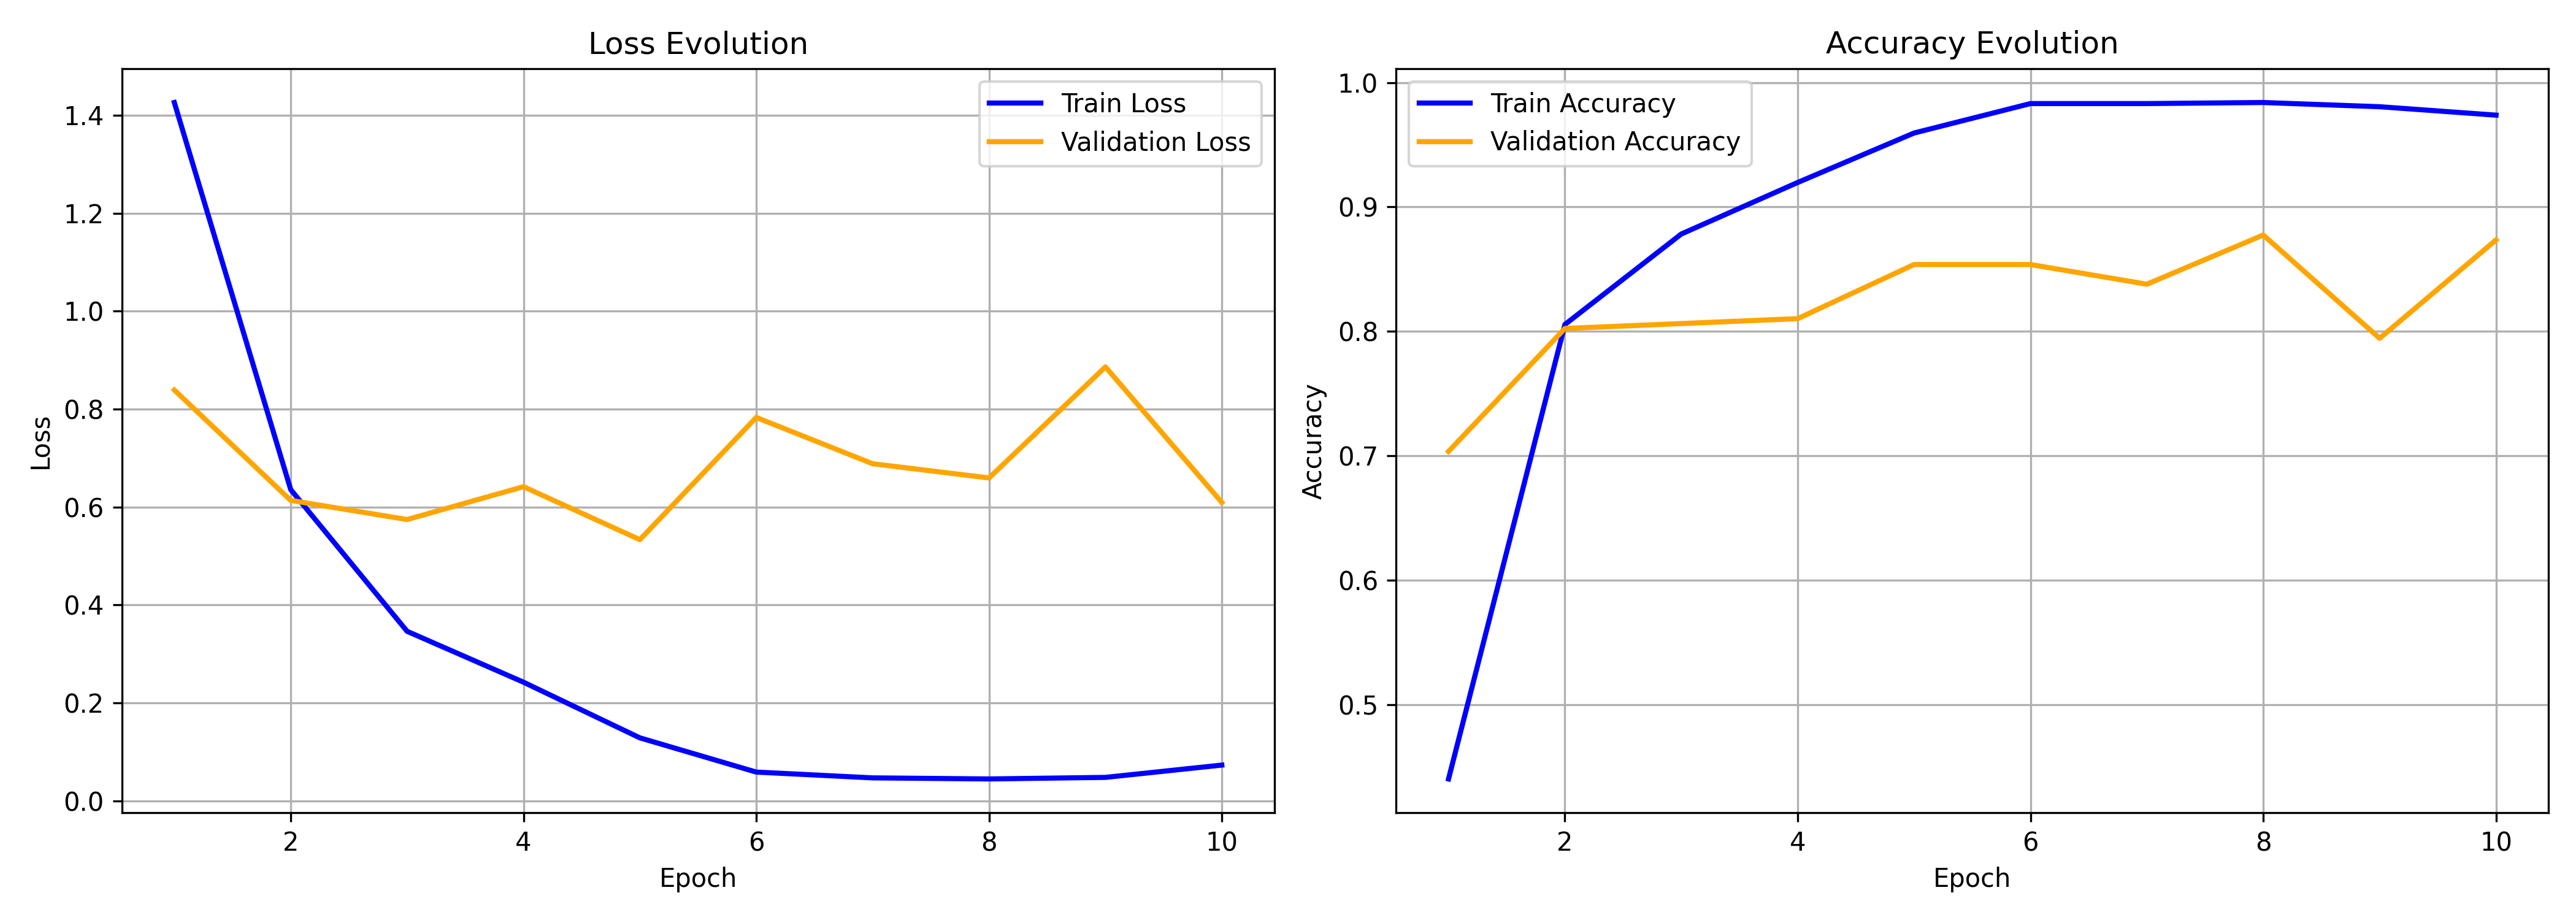
\includegraphics[width=0.90\linewidth]{../results/config7_normalize/training_history.png}
\caption{Evolución de la pérdida y precisión en entrenamiento y validación (Experimento 7). La red aprende y memoriza mucho antes que en cualquier configuración anterior, y la pérdida de validación se estabiliza en valores bajos desde la primera época.}
\label{fig:curvas_exp7}
\end{figure}

\subsubsection{Un efecto enorme en la convergencia}

Algo curioso de este experimento no es su resultado final sino la velocidad a la que llega a él. En la \textbf{primera época}, la precisión de validación alcanza el \textbf{70.36\%}. Las otras tres configuraciones que comparten con ella el tamaño de lote y la tasa de aprendizaje, y que difieren únicamente en que no normalizan, obtienen en esa misma época un 31.62\% (Experimento 3), un 56.52\% (Experimento 5) y un 34.39\% (Experimento 6). La normalizada casi duplica a las demás en el mismo número de iteraciones, y supera incluso resultados finales de algunas de ellas.

La explicación está en cómo se inicializan los pesos. Todos los pesos se sortean con una distribución centrada en cero, de modo que si las entradas están en $[0, 1]$ y con media muy positiva, las primeras capas reciben activaciones desplazadas y los gradientes resultantes están mal condicionados desde el principio.

\subsubsection{Resultado y significancia}

La precisión en el conjunto de prueba es del \textbf{88.98\%}, con 226 aciertos sobre 254, lo que la empata con el Experimento 2 y la sitúa tercera del ranking hasta ahora. Frente al modelo base la diferencia es de \textbf{solo tres imágenes}, tampoco significativa con este tamaño de datos.

\subsection{Experimento 8: aumentación de datos}

Los siete experimentos anteriores entrenan siempre sobre las mismas 1183 imágenes, transformadas de forma idéntica en cada época. Este experimento ataca esa limitación directamente, sin conseguir ni una sola imagen nueva, mediante \textbf{data augmentation}: se aplican transformaciones aleatorias al conjunto de entrenamiento para que la red vea en cada época una versión ligeramente distinta de cada imagen.

Las cuatro transformaciones empleadas se aplican solo durante el entrenamiento:

\begin{itemize}
    \item \textbf{Volteo horizontal} (\texttt{RandomHorizontalFlip}, $p = 0.5$): la mitad de las veces el vehículo aparece en espejo. Un coche visto desde un lado y desde el otro sigue siendo un coche.
    \item \textbf{Rotación aleatoria} (\texttt{RandomRotation}, $\pm 15^{\circ}$): simula la inclinación con la que puede estar tomada la foto.
    \item \textbf{Traslación} (\texttt{RandomAffine}, desplazamiento del 10\%): el vehículo puede aparecer descentrado dentro del encuadre.
    \item \textbf{Variación de color} (\texttt{ColorJitter}, brillo, contraste y saturación con factor 0.2): absorbe diferencias de iluminación y de exposición entre fotos.
\end{itemize}

Se descartaron deliberadamente el volteo vertical, porque un vehículo boca abajo no es un vehículo, y los recortes agresivos, porque un recorte profundo puede recortar el objeto entero o gran parte de él y dejar la etiqueta sin sentido.

Estas transformaciones afectan \textbf{exclusivamente al conjunto de entrenamiento}. El conjunto de validación y el de prueba se procesan igual que siempre, con el pipeline limpio. 

\begin{table}[H]
\centering
\caption{Métricas obtenidas en el Experimento 8 (aumentación de datos), medidas sobre los pesos de la época 34.}
\label{tab:resultados_exp8}
\begin{tabular}{l c c}
\toprule
\textbf{Conjunto de Datos} & \textbf{Pérdida (Loss)} & \textbf{Precisión (Accuracy)} \\
\midrule
Entrenamiento & 0.1911 & 93.58\% \\
Validación & 0.2506 & 94.47\% \\
\textbf{Prueba (Test)} & \textbf{0.2666} & \textbf{91.73\%} \\
\bottomrule
\end{tabular}
\end{table}

\begin{figure}[H]
\centering
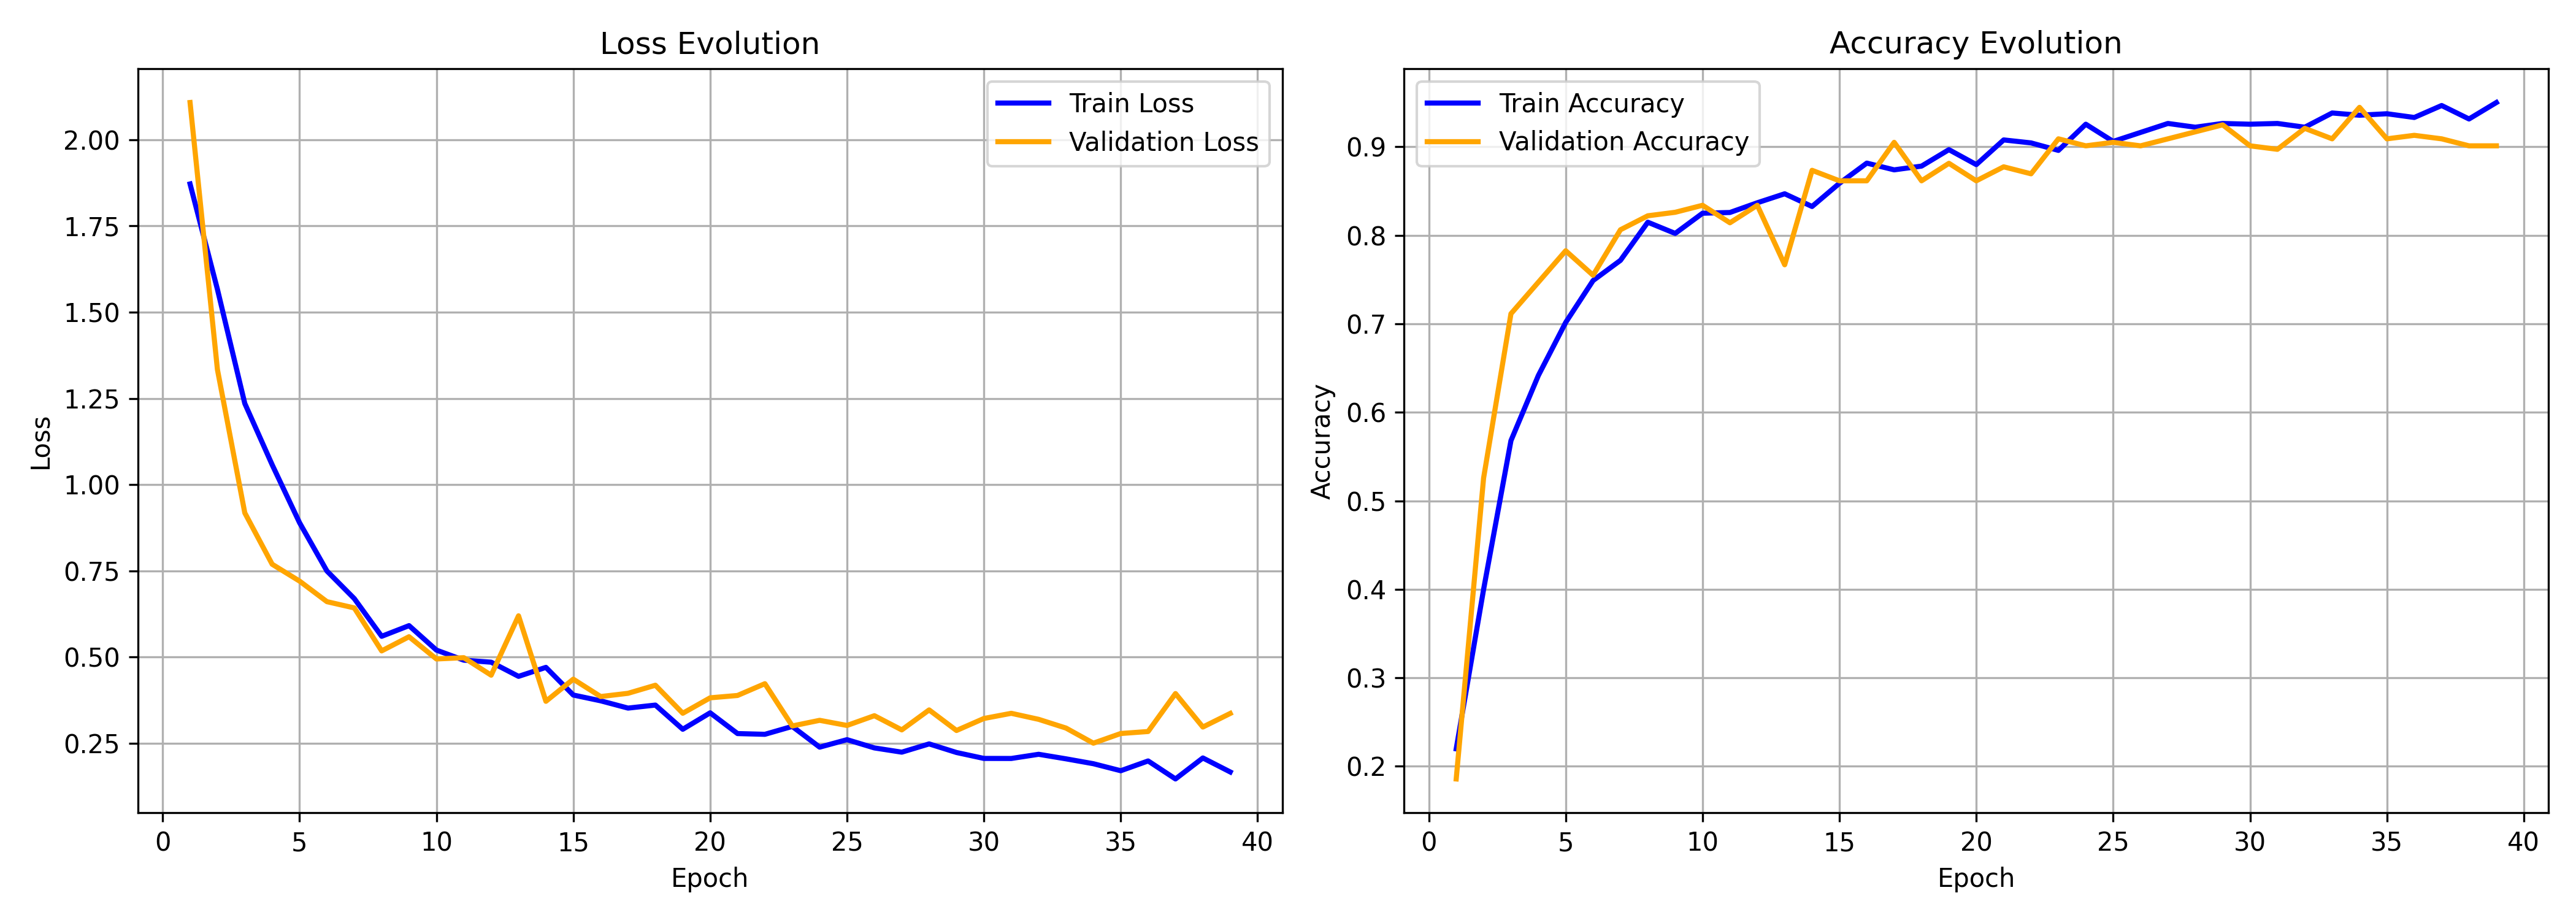
\includegraphics[width=0.90\linewidth]{../results/config8_augmented/training_history.png}
\caption{Evolución de la pérdida y precisión en entrenamiento y validación (Experimento 8). Nótese que la curva de validación acompaña a la de entrenamiento durante toda la ejecución, y que el entrenamiento dura casi cuatro veces más que en cualquier configuración anterior.}
\label{fig:curvas_exp8}
\end{figure}

\begin{figure}[H]
\centering
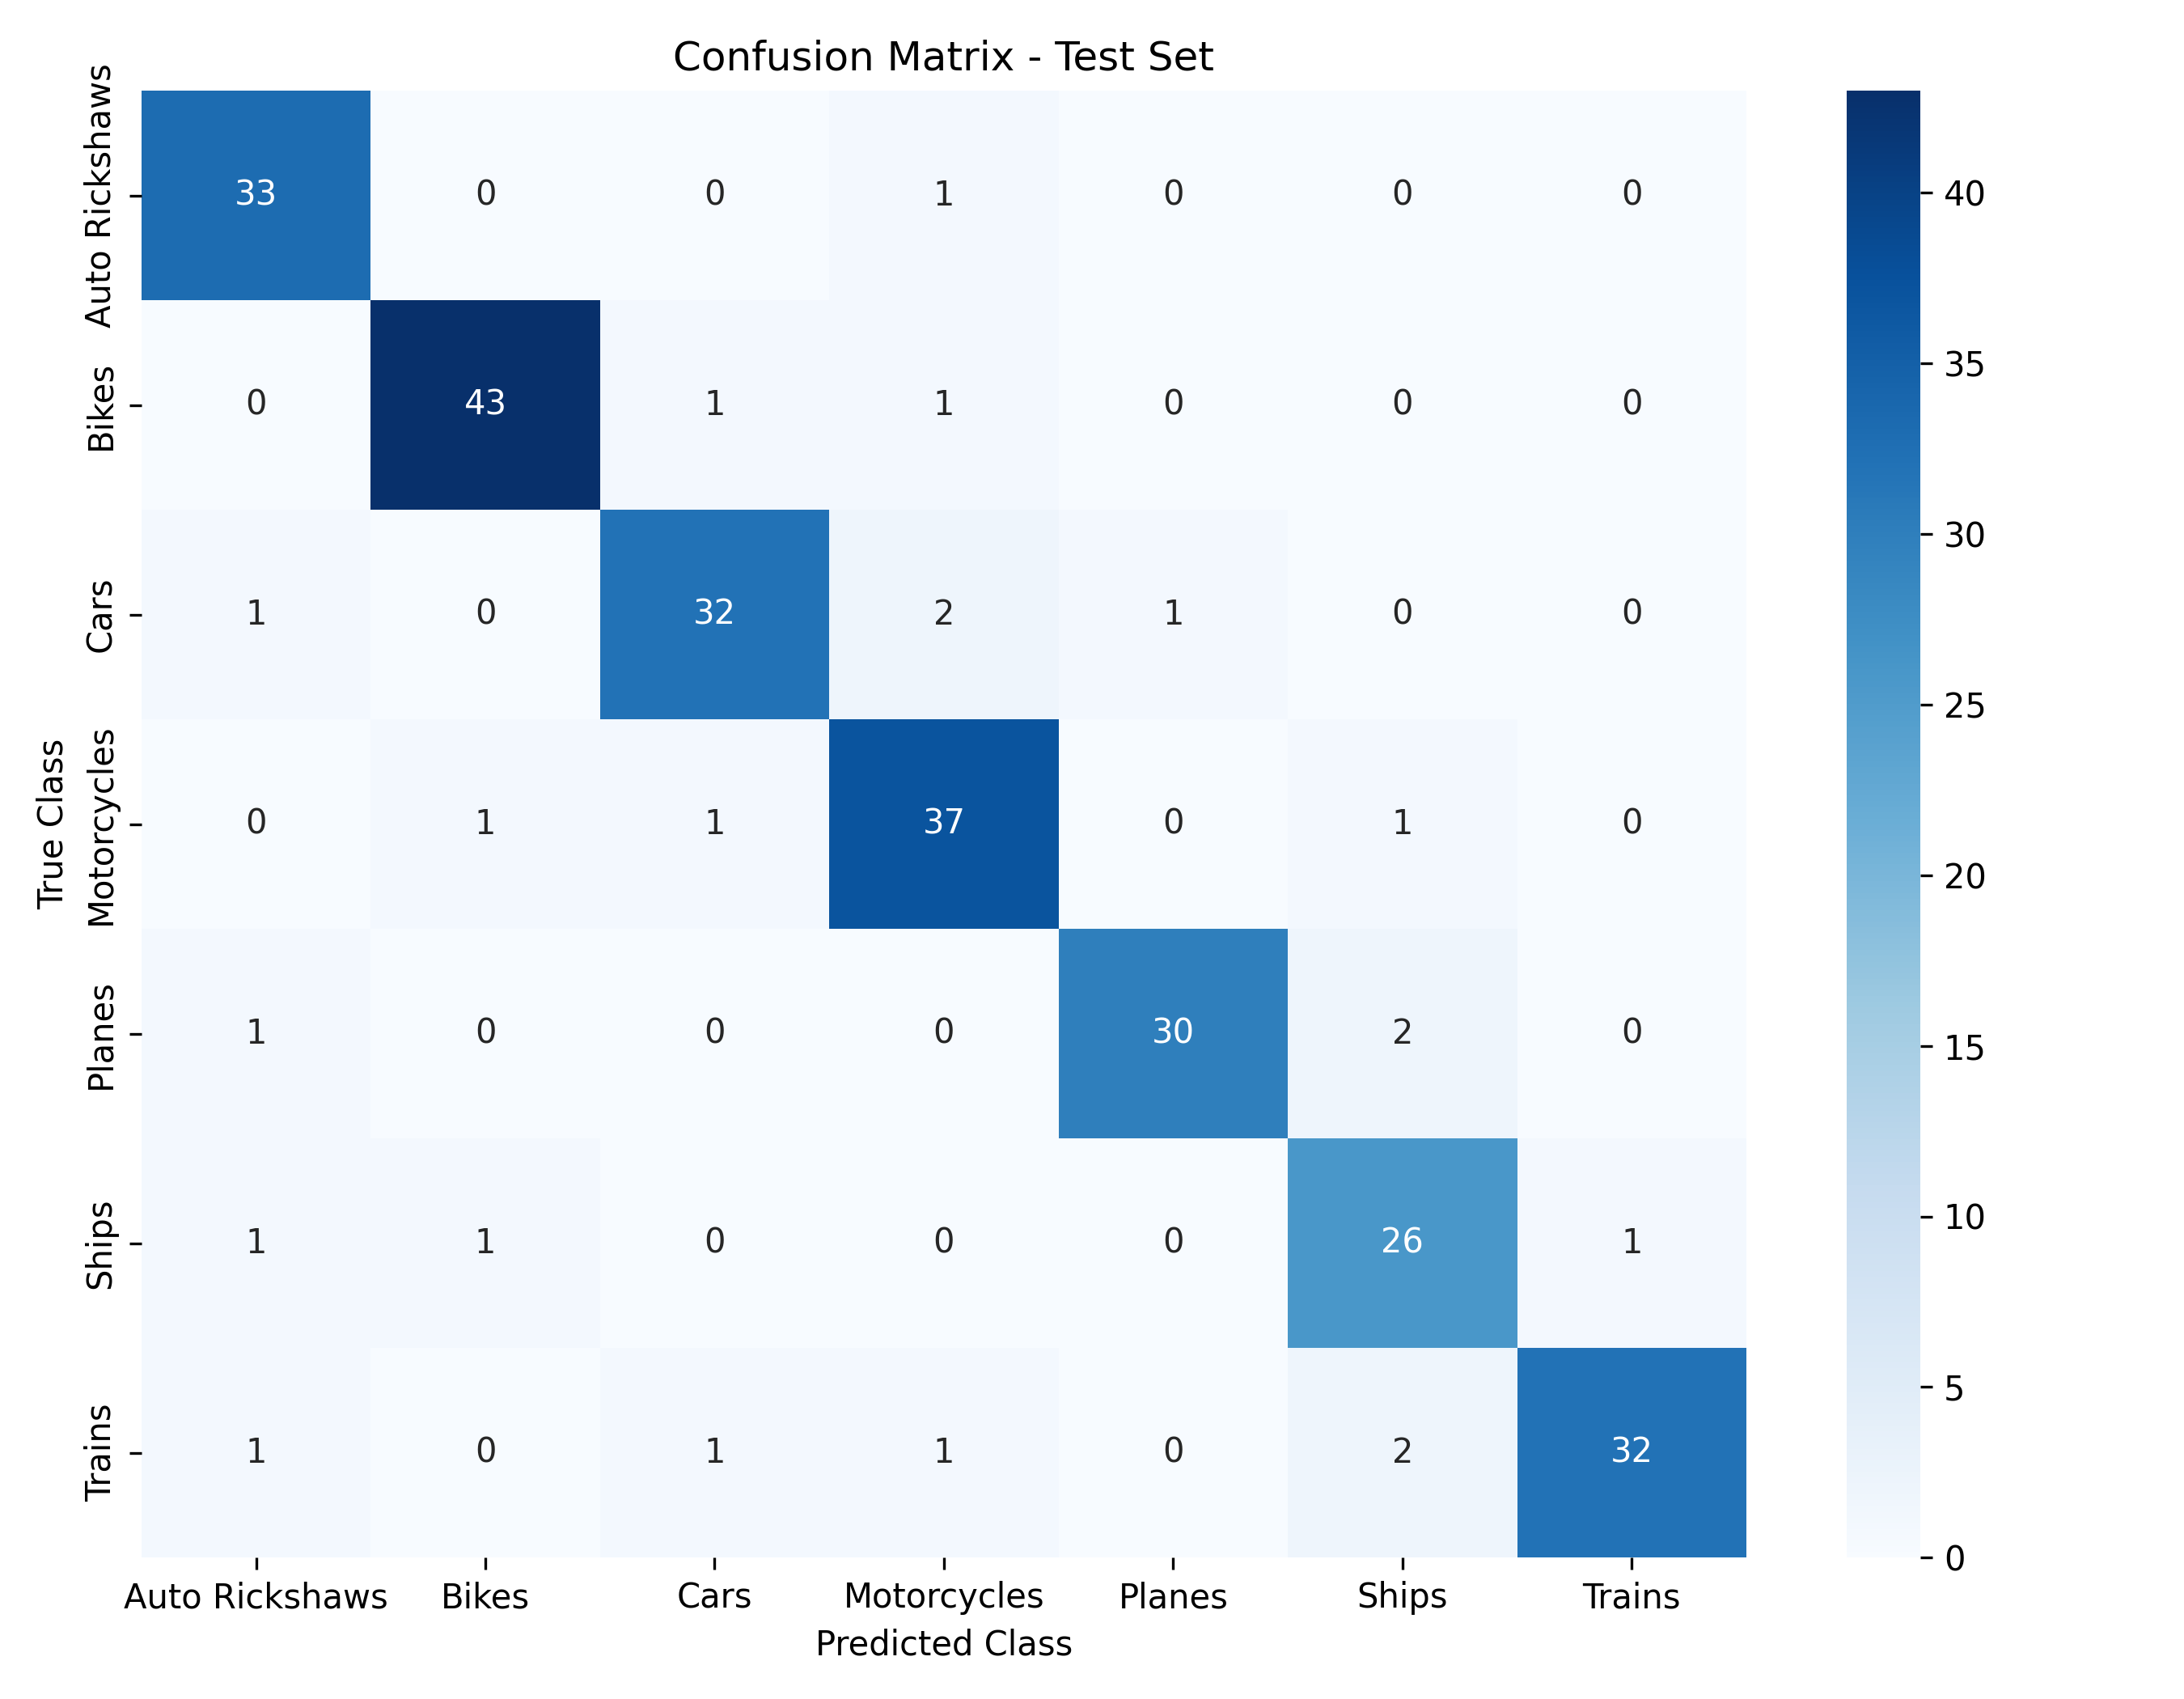
\includegraphics[width=0.65\linewidth]{../results/config8_augmented/test_confusion_matrix.png}
\caption{Matriz de confusión sobre el conjunto de prueba (Experimento 8). Las clases peor resueltas siguen siendo las de fondos dominantes, \textit{ships} y \textit{planes}, cuya textura de agua y de cielo resulta difícil de separar.}
\label{fig:matriz_exp8}
\end{figure}

\subsubsection{El sobreajuste desaparece}

La consecuencia más visible de la aumentación es la que se esperaba: la red tarda mucho más en memorizar. El entrenamiento se prolonga hasta la \textbf{época 39}, frente a las 10 a 14 épocas de casi todas las configuraciones anteriores, y la precisión de entrenamiento en el punto óptimo, 93.58\%, queda \textbf{por debajo} de la de validación, 94.47\%. La brecha entre ambos conjuntos, que en las siete configuraciones previas iba de $-4.00$ a $+11.87$ puntos, aquí es de \textbf{$-0.89$}: lo que sugiere ausencia de sobreajuste.

La razón es que el modelo ya no puede memorizar las imágenes porque, cada vez que las ve, las ve distintas.

\subsubsection{Análisis de la pérdida}

La precisión en el conjunto de prueba sube al \textbf{91.73\%}, con 233 aciertos sobre 254, lo que la convierte en la mejor del estudio. Pero la cifra que separa a esta configuración del resto no es esa, sino la \textbf{pérdida}:

\begin{itemize}
    \item Pérdida de validación mínima alcanzada: \textbf{0.2506}. La siguiente mejor de todo el estudio es 0.3839, la del Experimento 3.
    \item Pérdida sobre el conjunto de prueba: \textbf{0.2666}. La siguiente mejor es 0.3595, la del Experimento 4.
\end{itemize}

Es una reducción del \textbf{35\%} y del \textbf{26\%} respectivamente. La precisión, en cambio, solo suma tres imágenes sobre el Experimento 4. La diferencia entre ambas métricas es importante: la \textbf{precisión} solo cuenta aciertos y errores, y trata por igual una predicción dudosa que resulta acertada y una predicción correcta pero precaria. La \textbf{pérdida} mide además la \textbf{confianza} con la que el modelo la emitió. Una pérdida mucho menor con una precisión parecida significa que la red acierta con más holgura y, sobre todo, que sus errores son 'mejores': cuando se equivoca, no lo hace convencida.

\subsection{Experimento 9: aprendizaje por transferencia}

Los ocho experimentos anteriores entrenan una red desde cero. Este noveno y último plantea la pregunta que venía quedando en el aire tras el Experimento 6: si la red tiene capacidad de sobra pero no le bastan los datos para aprovecharla, ¿y si el problema no es la cantidad de datos sino que la red tiene que aprender demasiadas cosas a la vez?

Nuestra red convolucional actual entrenada desde cero tiene que descubrir por su cuenta, a partir de 1183 imágenes, dos tareas simultáneamente: \textbf{cómo mirar} (detectar bordes, texturas, contornos y formas) y \textbf{qué distinguir} (diferenciación entre las distintas clases). Son muchas cosas para tan pocas muestras. El aprendizaje por transferencia separa las dos: se parte de una red ya entrenada y se reutiliza su forma de 'mirar', dejando que el conjunto de entrenamiento se ocupe solo de la segunda tarea.

La red elegida es \textbf{ResNet-18}, preentrenada sobre \textbf{ImageNet}, un conjunto de 1,28 millones de imágenes distribuidas en 1000 clases. El tratamiento aplicado es el siguiente:

\begin{itemize}
    \item Se \textbf{congela} todo el backbone: a sus parámetros se les pone \texttt{requires\_grad = False} y no se actualizan en ningún momento.
    \item Se \textbf{sustituye} la capa de salida original, que clasificaba en 1000 clases, por una nueva de $512 \rightarrow 7$ (adaptada a nuestro problema).
    \item Se entrena \textbf{únicamente} esa capa nueva.
\end{itemize}

El balance de parámetros es el argumento entero del experimento:

\begin{table}[H]
\centering
\caption{Comparación de parámetros entre el modelo base y la configuración 9.}
\label{tab:parametros_transfer}
\begin{tabular}{l r r}
\toprule
\textbf{Modelo} & \textbf{Parámetros totales} & \textbf{Parámetros entrenables} \\
\midrule
ConvNet (Experimento 1) & 1.245.991 & 1.245.991 \\
ResNet-18 (Experimento 9) & 11.180.103 & \textbf{3.591} \\
\bottomrule
\end{tabular}
\end{table}

La red del Experimento 9 es, en total, casi nueve veces más grande que la del modelo base, pero \textbf{entrena 347 veces menos parámetros}. Los 11.176.512 pesos congelados no son trabajo del experimento: ya vienen hechos.

Durante el experimento, se han llevado a cabo 2 ajustes necesarios. El primero es la \textbf{resolución}: ResNet-18 fue diseñada con entradas de $224 \times 224$, de modo que las imágenes se redimensionan a ese tamaño en lugar de los $96 \times 96$ de los experimentos anteriores. El segundo es la \textbf{normalización}, que en este caso no es opcional sino exigida por la red: se usan las medias y desviaciones de ImageNet, exactamente las mismas que se emplearon en el Experimento 7. Esos dos cambios son precisamente el motivo de haber aislado la normalización en un experimento propio, en lugar de incluirla directamente aquí: de ese modo, si la configuración 9 mejora, la mejora se atribuye al modelo preentrenado y no al preprocesamiento que lo acompaña.

Existe además un matiz de implementación que no es un detalle menor. Las capas \texttt{BatchNorm}, presentes en ResNet-18, se comportan de forma distinta según el modo en que se ejecuta la red: en modo entrenamiento recalculan sus estadísticas con cada lote, y en modo evaluación usan las que traían guardadas. Congelar los pesos de estas capas \textbf{no basta}, porque aunque sus pesos no se actualicen, sus estadísticas sí lo harían, y con 1183 imágenes se corromperían. Por eso, tras activar el modo entrenamiento de la red, se fuerza el modo evaluación sobre el backbone en cada época. Se ha verificado el efecto y sin esa línea, las estadísticas cambian con cada lote; con ella permanecen intactas.

\begin{table}[H]
\centering
\caption{Métricas obtenidas en el Experimento 9 (aprendizaje por transferencia), medidas sobre los pesos de la época 50.}
\label{tab:resultados_exp9}
\begin{tabular}{l c c}
\toprule
\textbf{Conjunto de Datos} & \textbf{Pérdida (Loss)} & \textbf{Precisión (Accuracy)} \\
\midrule
Entrenamiento & 0.0012 & 100.00\% \\
Validación & 0.0053 & 100.00\% \\
\textbf{Prueba (Test)} & \textbf{0.0129} & \textbf{99.61\%} \\
\bottomrule
\end{tabular}
\end{table}

\begin{figure}[H]
\centering
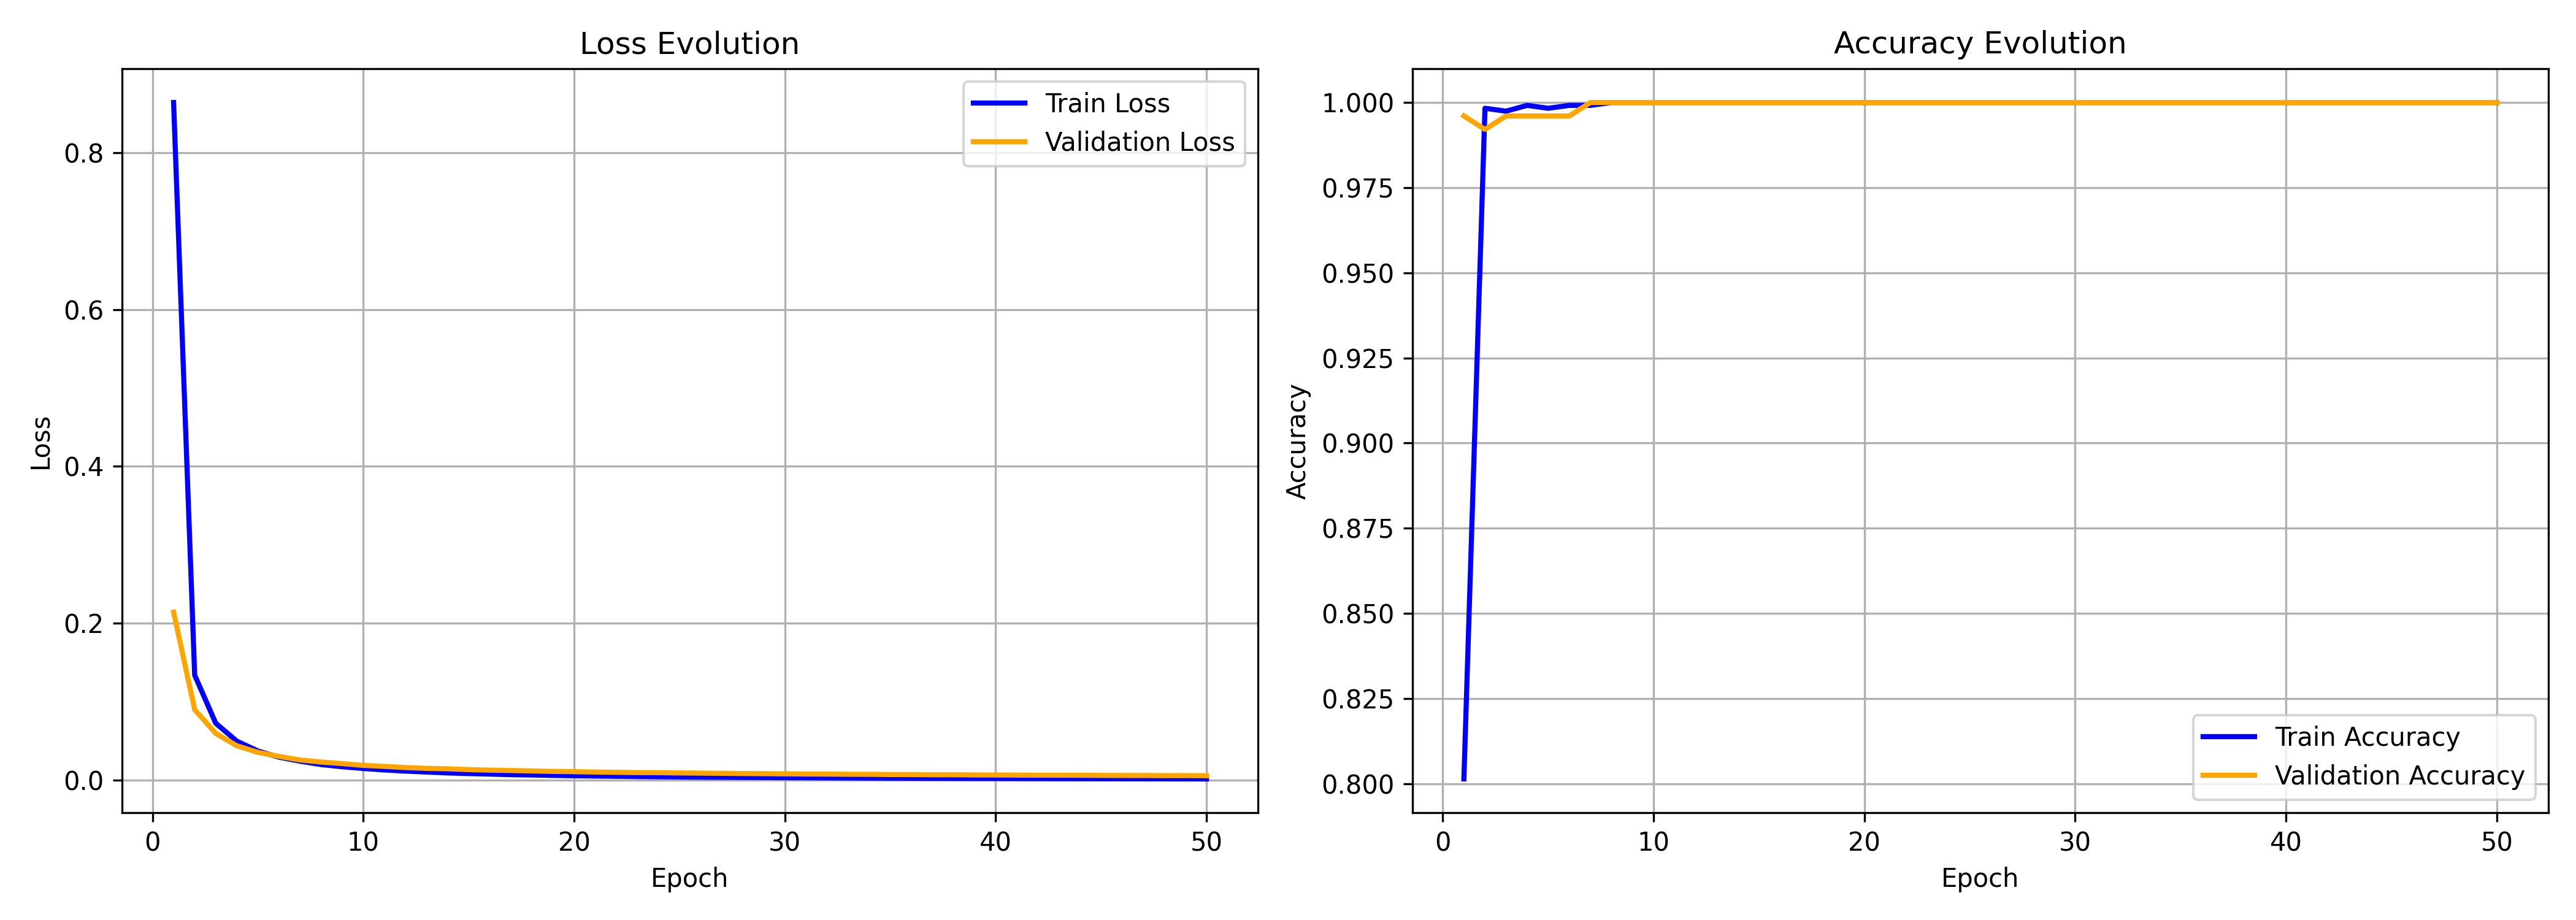
\includegraphics[width=0.90\linewidth]{../results/config9_transfer/training_history.png}
\caption{Evolución de la pérdida y precisión en entrenamiento y validación (Experimento 9). La precisión se sitúa en el 99.6\% ya en la primera época y la pérdida de validación desciende sin estancarse durante las 50 épocas completas, de modo que la parada anticipada nunca llega a intervenir.}
\label{fig:curvas_exp9}
\end{figure}

\begin{figure}[H]
\centering
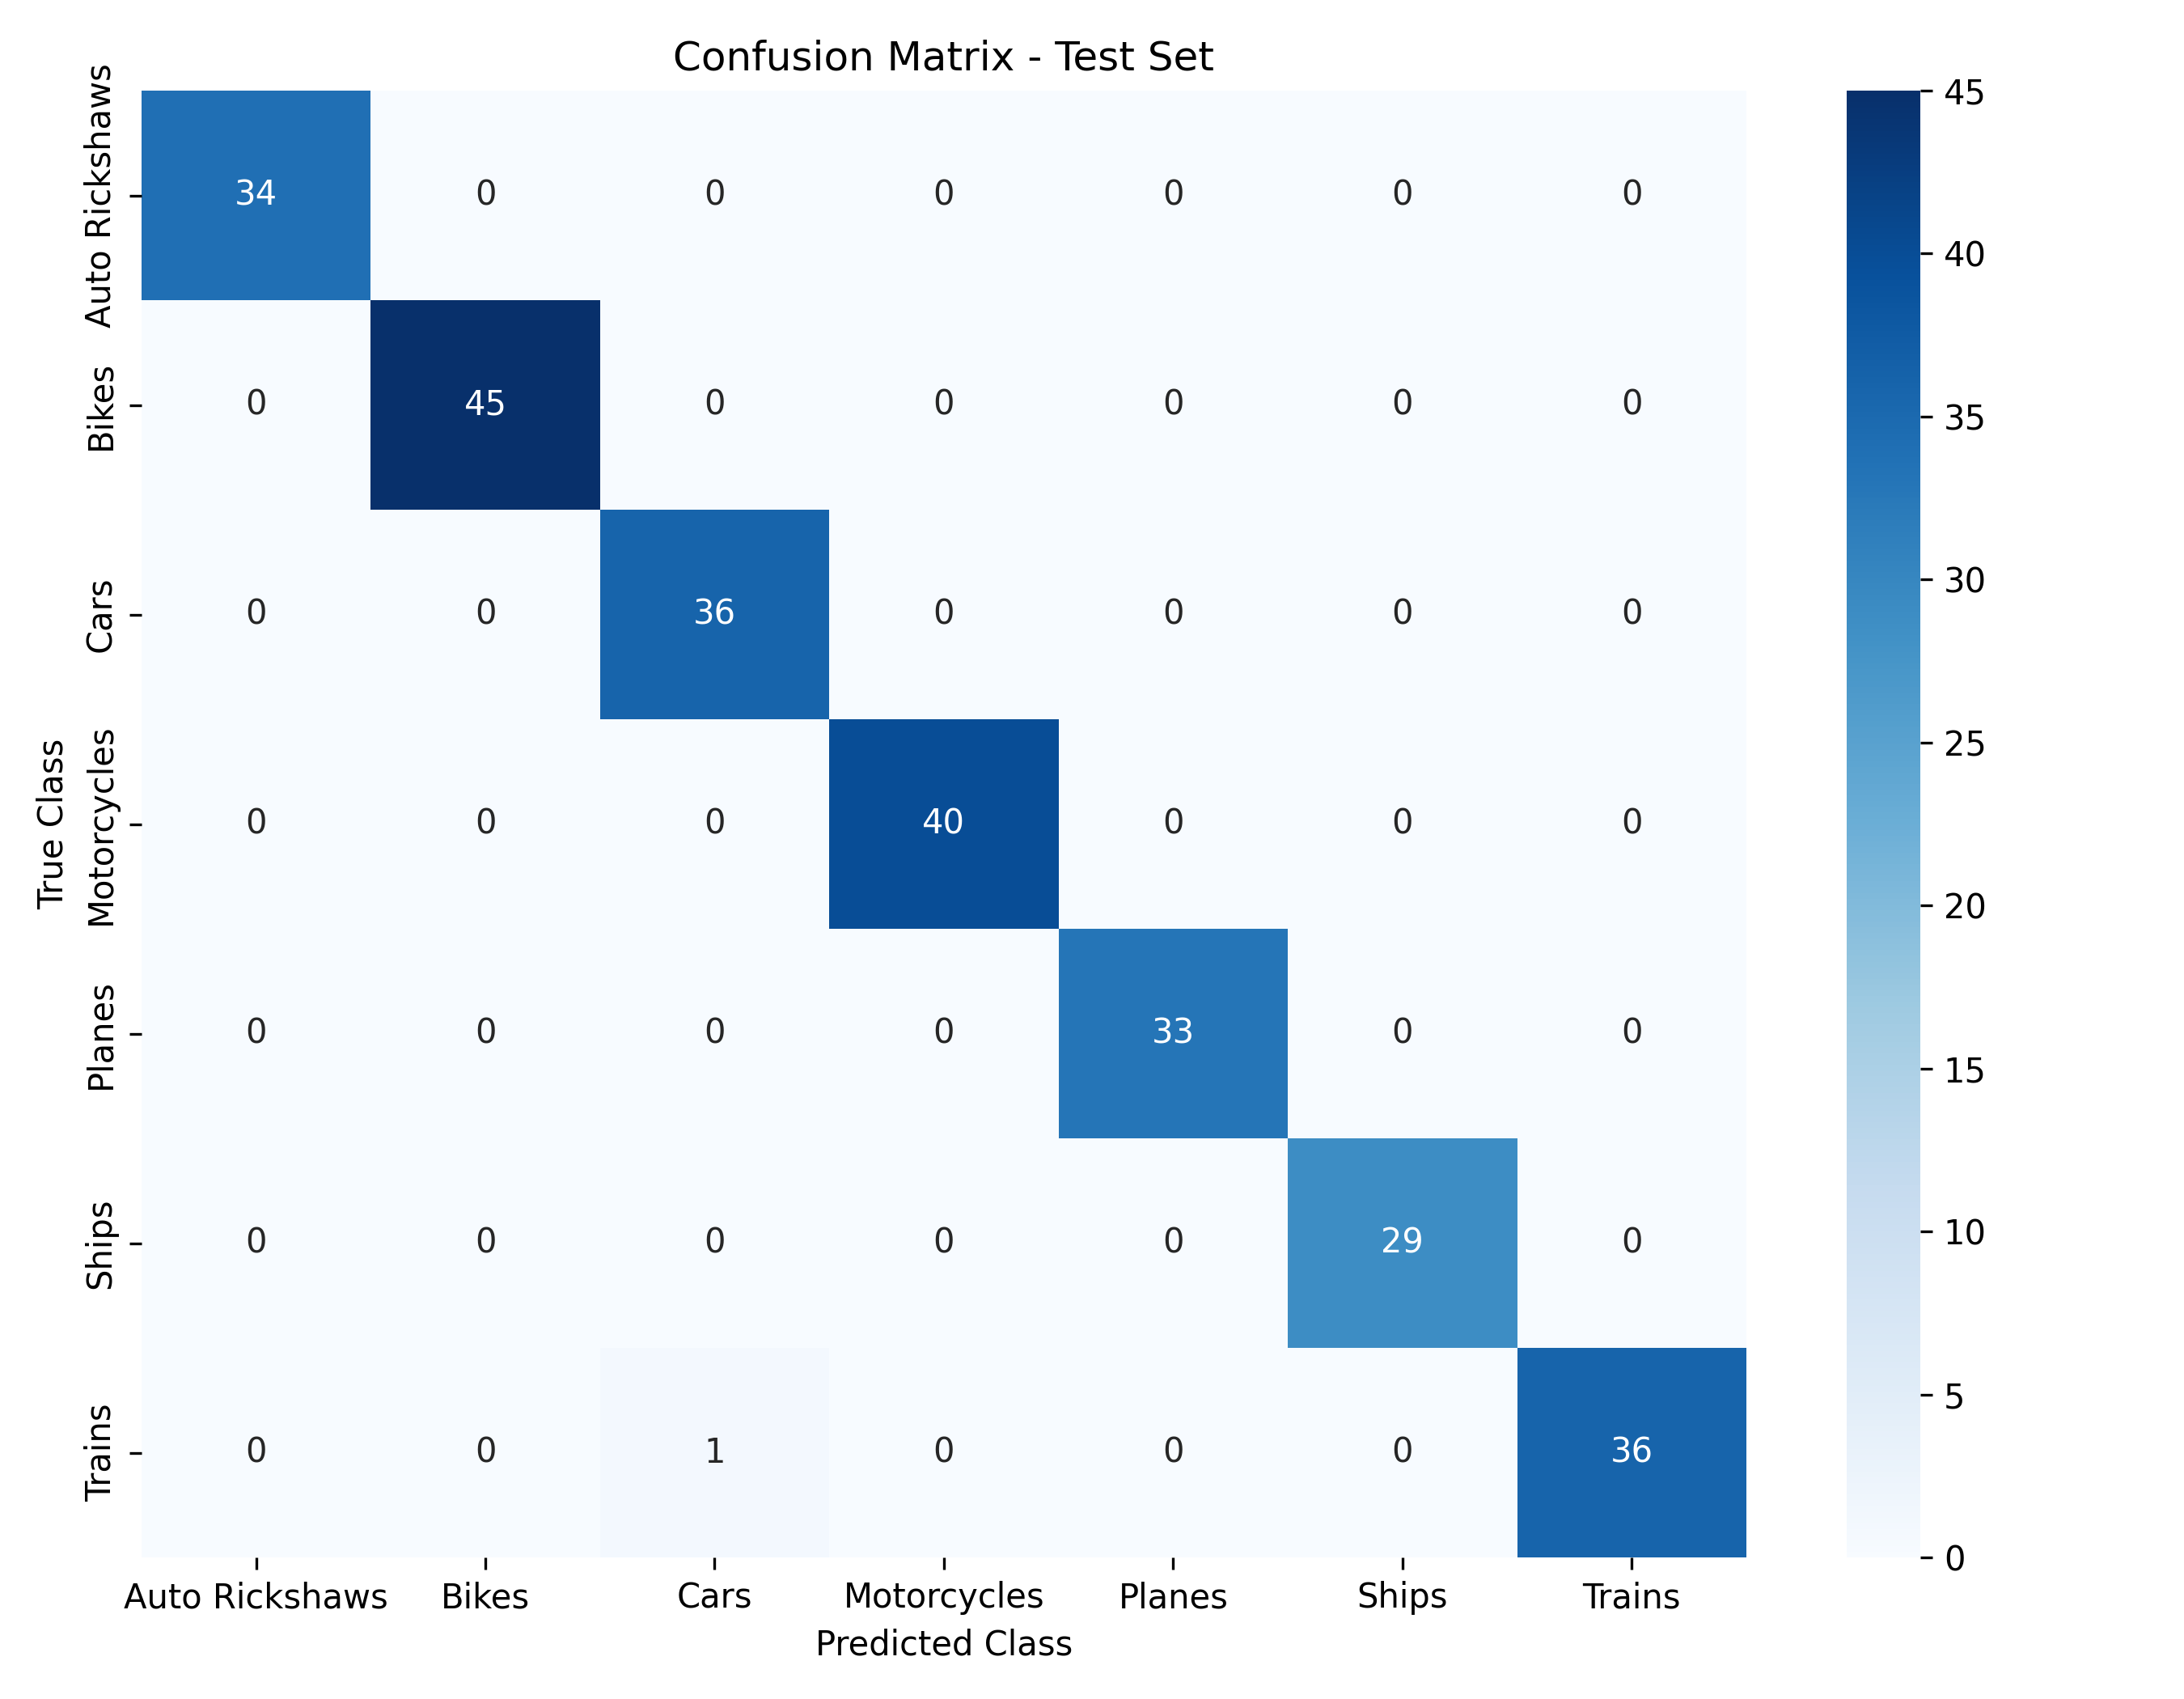
\includegraphics[width=0.65\linewidth]{../results/config9_transfer/test_confusion_matrix.png}
\caption{Matriz de confusión sobre el conjunto de prueba (Experimento 9). De las 254 imágenes, 253 se clasifican correctamente y solo una falla.}
\label{fig:matriz_exp9}
\end{figure}

\subsubsection{El resultado}

La precisión sobre el conjunto de prueba es del \textbf{99.61\%}: \textbf{253 aciertos de 254}, con una sola imagen mal clasificada. La pérdida de prueba, 0.0129, es \textbf{veinte veces menor} que la de la mejor configuración anterior, la del Experimento 8 con 0.2666.

La velocidad es tan llamativa como el resultado. La precisión de validación alcanza el \textbf{99.60\%} en la \textbf{primera época}: con la capa de salida apenas entrenada, las características preentrenadas ya separan las siete clases casi sin esfuerzo. En el resto del entrenamiento, la pérdida de validación desciende de 0.2140 a 0.0053 \textbf{sin estancarse en ninguna de las 50 épocas}, de modo que la parada anticipada nunca se activa y el modelo llega al tope de épocas. Es el único experimento de los nueve en el que el entrenamiento no se interrumpe por sí mismo.

Tampoco hay sobreajuste: la precisión de entrenamiento y la de validación coinciden ambas en el 100\%. La brecha entre conjuntos se reduce a cero.

\section{Conclusiones}

\paragraph{El cuello de botella nunca fue la arquitectura, sino la representación.}
Los ocho primeros experimentos ajustan la red: profundidad, activación, tamaño de lote, etc. Ninguno consigue una mejora demostrable, y el mejor apenas suma siete imágenes sobre el modelo base. El noveno no modifica ninguno de esos parámetros, sino lo que la red \textbf{sabe} antes de empezar, y suma veinte imágenes sobre el mejor de los anteriores.

Por tanto, la lectura correcta \textbf{no} es que únicamente faltaran datos. El Experimento 9 entrena sobre \textbf{exactamente las mismas 1183 imágenes} que el modelo base, y con las mismas etiquetas. Lo que cambia es que una red entrenada desde cero tiene que hacer dos trabajos a la vez: descubrir \textbf{cómo mirar} y aprender \textbf{qué distinguir}, y 1183 imágenes no dan para las dos cosas. Con la forma de mirar ya resuelta, esas 1183 imágenes se dedican enteras a la segunda tarea, que es mucho más fácil. La red del Experimento 9 entrena 347 veces menos parámetros que la del modelo base y lo hace incomparablemente mejor.

El trabajo cumple los objetivos planteados. El clasificador alcanza un \textbf{99.61\% de precisión} sobre el conjunto de prueba con la configuración 9, que se traduce en \textbf{253 aciertos de 254 imágenes}, superando de largo el 85\% exigido. Se han comparado un total de \textbf{nueve configuraciones} organizadas en dos fases: una búsqueda de hiperparámetros sobre la arquitectura base y un segundo bloque sobre los datos de entrada y el propio modelo. La parada anticipada basada en la pérdida de validación se ha empleado en todas ellas y ha resultado indispensable: en los ocho primeros casos el modelo habría seguido memorizando el conjunto de entrenamiento sin mejorar la generalización.

\begin{table}[H]
\centering
\caption{Ranking final de las nueve configuraciones ordenado por precisión sobre el conjunto de prueba.}
\label{tab:ranking}
\footnotesize
\setlength{\tabcolsep}{3pt}
\begin{tabular}{c l r c c c}
\toprule
\textbf{Pos.} & \textbf{Configuración} & \textbf{Prec. Test} & \textbf{Aciertos} & \textbf{Pérdida} & \textbf{Brecha tr./val.} \\
\midrule
1 & 9 --- aprendizaje por transferencia & \textbf{99.61\%} & 253/254 & \textbf{0.0129} & \textbf{0.00} \\
2 & 8 --- aumentación de datos & 91.73\% & 233/254 & 0.2666 & -0.89 \\
3 & 4 --- tamaño de lote 64 & 90.55\% & 230/254 & 0.3595 & +7.10 \\
4 & 2 --- tasa de aprendizaje $10^{-4}$ & 88.98\% & 226/254 & 0.3778 & +9.38 \\
5 & 7 --- normalización de píxeles & 88.98\% & 226/254 & 0.3779 & +10.56 \\
6 & 1 --- modelo base & 87.80\% & 223/254 & 0.4141 & +3.39 \\
7 & 5 --- \texttt{LeakyReLU} & 87.01\% & 221/254 & 0.4736 & +11.87 \\
8 & 3 --- cuatro capas convolucionales & 84.25\% & 214/254 & 0.6654 & +8.90 \\
9 & 6 --- capa densa de 32 neuronas & 83.07\% & 211/254 & 0.5205 & -4.00 \\
\bottomrule
\end{tabular}
\setlength{\tabcolsep}{6pt}
\end{table}

\end{document}